\documentclass[11pt, a4paper, openright, titlepage, final, language = italian]{book}
% draft/final onecolumn/twocolumn oneside/twoside openany/openright  
% Circa 80 lettere per pagina con draft al posto di final fa il pdf senza foto
\usepackage[toc,page]{appendix}

\usepackage[english, italian]{babel} % per la sillabazione corretta e per biblatex
% \usepackage[english]english serve se c'e' bisogno di una parte da scriver ion inglese

% https://tex.stackexchange.com/questions/82993/how-to-change-the-name-of-document-elements-like-figure-contents-bibliogr

\usepackage[sc]{mathpazo}
\usepackage[T1]{fontenc}
\usepackage[utf8]{inputenc}
% \usepackage{geometry}
% \geometry{verbose,tmargin=2.5cm,bmargin=2.5cm,lmargin=2.5cm,rmargin=5cm}
% \usepackage[nochapters,pdfspacing,dottedtoc]{classicthesis}
% \setcounter{secnumdepth}{4} % numerini alle sezioni dentro al testo
% \setcounter{tocdepth}{4} % nell'indice
\usepackage{url}
\usepackage{comment}

% hyperref serve per i link
% Tutti le opzioni che ci sono adesso non sappiamo se servono: le disattivo per il momento
% 
\usepackage[]{hyperref} % caricare questo prima di floats per evitare casini
% unicode=true, pdfusetitle, backref=false, pdfborder={0 0 1},
% bookmarks=true, bookmarksnumbered=true, bookmarksopen=true, bookmarksopenlevel=2, colorlinks=false,
% breaklinks=false

%% xcolor serve per colorare il testo
\usepackage[dvipsnames]{xcolor}
%% Questa parte sotto controlla i colori dei riferimenti cliccabili
\hypersetup{colorlinks,
  linkcolor={red!50!black},
  citecolor={red},
  urlcolor={blue!80!black},
  pdfstartview={XYZ null null 1}
}
% \usepackage{textcomp}
% Sperimentale per le liste; non attivare
%% \usepackage{enumitem}
%% \setlist{nosep} %

\usepackage{longtable} % per avere tabelle spezzate tra le pagine
\usepackage{tabularx} % per le tabelle con molto testo
\usepackage{lscape} % per ruotare qualche pagina in landscape
\usepackage{booktabs} % per fare tabelle semplici come nei libri (top mid e bottomrule)

\usepackage{setspace} % permette di cambiare la spaziatura quando necessario
%\doublespacing % per avere spazio per scrivere a penna
\onehalfspacing  % per l'interlinea finale
% meglio questi due comandi sopra che linespread.
% Cosi sistema interlinea 1 nelle tabelle automaticamente
% \linespread{1.3} % Di default è \linespread{1} che corrisponde
% all'interlinea uno; 1.3 sta per interlinea 1 e mezzo

%% \usepackage{multirow} % tabelle multiriga e multicolonna

%% \usepackage{threeparttable}
% vedi http://www.tug.org/pracjourn/2007-2/asknelly/

%% \usepackage{lineno}
%% \linenumbers
% Queste due righe sopra aggiungono la numerazione delle righe
% scommentare nella versione finale

% Queste righe sotto si occupano della bibliografia
\usepackage[babel]{csquotes}
\usepackage[backend=biber, sorting=nyt, style=authoryear, autolang=hyphen, natbib=true, backref]{biblatex}
%% style=numeric

% nty Sort by name, title, year.
% nyt Sort by name, year, title.
% nyvt Sort by name, year, volume, title.
% anyt Sort by alphabetic label, name, year, title.
% anyvt Sort by alphabetic label, name, year, volume, title.
% ynt Sort by year, name, title.
% ydnt Sort by year (descending), name, title.
% none Do not sort at all. All entries are processed in citation order.
% Debug Sort by entry key. This is intended for debugging only.

%% Qui sotto ci va il nome del file della bibliografia
\bibliography{bibliomone.bib}
% non ho capito a che serve ma dovrebbe essere utile a citare R in bib
% \newcommand{\code}[1]{\texttt{\smaller #1}}

%% siunitx serve per le unità di misura
\usepackage{siunitx}
\sisetup{detect-all = true, detect-family = true, output-decimal-marker = {,}}
% http://tex.stackexchange.com/questions/66713/can-i-make-siunitx-commands-use-serif-fonts-like-the-rest-of-the-math-in-beamer

%% questa roba sotto serve per non perdere il filo sulle copie stampate
%% commentare opportunamente nella versione finale
\usepackage[short, hhmmss]{datetime}
\usepackage{fancyhdr}
\usepackage{placeins}
\usepackage{graphicx} %per le figure
\pagestyle{fancy}
% \setlength{\headheight}{14pt} % il compilatore si lamenta che c'e' poco spazio 1 ott 2016 Siena
% \usepackage[]{subfig} % per le figure affiancate

\usepackage{float}
% per forzare il posizionamento delle figure

\usepackage[normalem]{ulem}
% serve per barrare del testo in fase di correzione
% se non si usa [normalem], \emph sottolinea invece di fare il suo dovere

%% Pezzo per scrivere note a margine
\usepackage{xargs} % Use more than one optional parameter in a new commands
\usepackage[colorinlistoftodos, prependcaption, italian, textsize=scriptsize]{todonotes}
\newcommandx{\dubbio}[2][1=]{\todo[linecolor=red,backgroundcolor=red!25,bordercolor=red,#1]{#2}}
\newcommandx{\cambia}[2][1=]{\todo[linecolor=blue,backgroundcolor=blue!25,bordercolor=blue,#1]{#2}}
\newcommandx{\info}[2][1=]{\todo[linecolor=OliveGreen,backgroundcolor=OliveGreen!25,bordercolor=OliveGreen,#1]{#2}}
\newcommandx{\migliora}[2][1=]{\todo[linecolor=Plum,backgroundcolor=Plum!25,bordercolor=Plum,#1]{#2}}
\newcommandx{\fatto}[2][1=]{\todo[linecolor=gray, backgroundcolor=black!75]{#2}}
\newcommandx{\nonvisibile}[2][1=]{\todo[disable,#1]{#2}}
%\presetkeys{todonotes}{fancyline}{}

\usepackage[raggedright]{titlesec} 
% Serve per evitare la sillabazione nei titoli

\newcommand{\sectionbreak}{\clearpage} 
%% serve per mettere ogni section a pagina nuova

\renewcommand{\chaptermark}[1]{\markboth{\thechapter.\space#1}{}}
\renewcommand{\headrulewidth}{0.4pt}
\renewcommand{\footrulewidth}{0.2pt}
% \cfoot{Pag. \thepage\, Compilata il \today\ alle \currenttime}
% \lfoot{}
% \rfoot{}
% E Even page
% O Odd page
% L Left field
% C Center field
% R Right field
% H Header
% F Footer
% \fancyhead{} % clear all header fields
\usepackage{enumitem} 
% per fare l'itemize con il tondo intorno ai numeri
% e altri controlli sulle liste

\usepackage{caption}


\DeclareCaptionFont{mysize}{\fontsize{10}{9.6}\selectfont}
\captionsetup{font=mysize}
% \usepackage[swapnames]{frontespizio} %per il frontespizio
\usepackage{frontespizio}

\newenvironment{abstract}%
{\cleardoublepage\null \vfill\begin{center}%
    \bfseries \abstractname \end{center} \footnotesize}%\doublespace }%
{\vfill\null}

\newenvironment{engabstract}%
{\cleardoublepage\null \vfill\begin{center}%
    \bfseries Summary  \end{center} \footnotesize}%\doublespace }%
{\vfill\null}

\usepackage[nogin]{Sweave}
% https://tex.stackexchange.com/questions/11619/resize-arrays-and-figures-in-a-sweave-document
% nogin serve per definiore le dimensioni delle figure e passarle a latex

\usepackage{lipsum}
% blocchi di testo fittizi



%%%%%%%%%%%%%%%%%%%%%%%%%%%%%%%%%%%%%%%%%%%%%%%%%%%%%%%%%%%%%%%%%%%%%%%%%%%%%%%%%%%%%%%%%%%%%%%%%%%%%%%%%%%% 
\author{Simone Massenzio}
\title{
  1) 30 anni di conduzione biologica: uno studio di fisica del
  suolo 
2) Trent'anni e non sentirli !!
3) Effetto di 30 anni di conduzione biologica sullo stato di
 aggregazione 
}
\begin{document}
% \begin{frontespizio}
%   \Universita{Università degli studi di Firenze}
%   \Facolta{Agraria}
%   
%   \Corso{Scienze e tecnologie agrarie}
%   \Annoaccademico{2016-2017}
%   \Titolo{Tesi di laurea magistrale}
%   %\Sottotitolo{Svolto da Simone Massenzio,\\ residente in Via don Minzoni 31A 59011 - Carmignano (PO), \\
% 	%	tel.: 3336277649, e-mail: simone.massenzio@stud.unifi.it\\ Svolto nel periodo compreso tra il 05/12/2016 e il 08/03/2017}
%   \NCandidato{Candidato}
%   \Candidato{Simone Massenzio}
%   \NRelatore{Relatore}{relatore}
%   \Relatore{Dott. Ottorino-Luca Pantani}
%   \NCorrelatore{Correlatore}{Correlatore}
%   \Correlatore{Dott. Luigi P. D'Acqui}
% \end{frontespizio}
\begin{frontespizio}
  \Margini{5cm}{1.5cm}{3cm}{1cm}
  \Logo[2.5cm]{logo-unifi_positivo.jpeg}
  \Istituzione{Universit\`a degli Studi di Firenze}
  \Divisione{Scuola di Agraria}
  \Scuola{Corso di Laurea in Scienze e tecnologie agrarie (LM-69)}
  \Titolo{
    1o) 30 anni (di conduzione biologica) e non sentirli ! Uno
    studio sullo stato di aggregazione del terreno   
    \newline
    2o) 30 anni di conduzione biologica: uno studio di fisica del
    suolo 
    \newline
    3o) Effetto di 30 anni di conduzione biologica sullo stato di
    aggregazione }
  \NCandidato{Candidato}
  \Candidato{Simone Massenzio}
  \NRelatore{Relatore}{}
  \Relatore{Dott. Ottorino-Luca Pantani}
  \NCorrelatore{Correlatori}{Correlatori}
  \Correlatore{Dott. Luigi Paolo D'Acqui}
  \Correlatore{Prof. Gaio Cesare Pacini}
  \Piede{Anno accademico 2016-2017}
\end{frontespizio}
%\maketitle



\begin{abstract}
  \lipsum[1-2]
\end{abstract}


\begin{otherlanguage*}{english}
\begin{engabstract}
  The purposes of this work were: \textbf{i)} to compare two farming
  systems (organic and conventional management on site since more than
  twenty years) through three soil's physical properties such as: bulk
  density, pore size distribution and aggregate stability.
  \textbf{ii)} to compare the effects of three tillage systems:
  plowing, chisel plowing and disk harrowing. The soil samples were
  taken in Montepaldi farm, situated in San Casciano val di Pesa
  (FI). The study is inserted in the MOLTE project, a long term
  experiment of the University of Florence where, since 1991, was
  carried out an experimentation on the organic farming systems.
  The results of the analysis of the bulk density, shows that there are
  statistically significant differences between the soil of the two
  farming systems, however these are not technologically significant. The
  results of the pore distribution are not statistically
  significant. The aggregate stability shows that the conventional's
  soil is more stable than the organic one. This could be due to the
  lack of fertilisation in the organic soil.
\end{engabstract}
\end{otherlanguage*}


\tableofcontents
\newpage
\fancyhead[RO,LE]{}
\fancyfoot{} % clear all footer fields
\fancyfoot[RE,LO]{Tesi Simone Massenzio}
\fancyfoot[C]{\today\  \currenttime}
\fancyfoot[LE,RO]{\thepage}

%%%%%%%%%%%%%%%%%%%%%%%%%%%%%%%%%%%%%%%%%%%%%%%%%%%%%%%%%%%%%%%%%%%%%%%%%%%%%%%%%%%%%%%%%%%%%%%%%%%%%%%%%%%% 

\chapter{Suolo agricolo e agricoltura biologica}
Il suolo o terreno \`e un concetto piuttosto chiaro nell'immaginario
collettivo; nonostante questo \`e difficile individuare una
definizione univoca. Un tentativo pu\`o essere quella data da
\citet{JOHNSON19986}: \textit{suolo è qualsiasi materiale minerale e
  organico posto alla superficie di pianeti o corpi simili, alterato
  da agenti biologici, chimici e/o fisici.} 

Nella definizione di Johnson non vengono considerate le piante; la
Soil Taxonomy ha fornito una definizione pi\`u completa in cui vengono
considerati anche gli organismi vegetali: \textit{Il suolo \`e un
  corpo naturale composto da una fase solida (minerale e organica),
  una fase liquida e una gassosa presenti sulla superficie terrestre,
  occupa spazio ed \`e caratterizzato da una o pi\`u delle seguenti
  caratteristiche: orizzonti, o strati, che sono distinguibili dal
  materiale iniziale grazie alle aggiunte, perdite, trasferimenti e
  trasformazioni di energia e materia o l'abilit\`a di supportare
  piante vascolari in un ambiente naturale} \citep{united1999soil}.

\dubbio{per ora non so cosa scriverci, mi verrà in mente qualcosa}

Dal suolo naturale distinguiamo il terreno agrario, questo è
caratterizzato da pesanti modifiche operate dall'uomo mediante
lavorazioni meccaniche, concimazioni e sistemazioni idrauliche.  Lo
scopo di queste operazioni è quello di aumentare il più possibile la
produzione alimentare umana e animale, mantenendo costante la
fertilit\`a del terreno.  

Secondo \citet{ellis1996soil}: \textit{la
  fertilit\`a di un suolo si riferisce all'abilit\`a di questo di
  fornire in maniera adeguata e proporzionata nutrienti e acqua
  necessari per la crescita e la riproduzione delle piante, e
  all'assenza di sostanze tossiche che possono inibirle.}

Tuttavia, lo sfruttamento intensivo del suolo degli ultimi 50 anni, ne ha
provocato la degradazione determinando una diminuzione della sua
fertilit\`a.

A fronte di un previsto aumento di popolazione, \`e pi\`u che mai
necessario cercare delle tecniche che permettano il mantenimento delle
caratteristiche dei terreni agrari senza diminuirne la
produttivit\`a. Gli stessi consumatori occidentali sono pi\`u attenti
ai loro acquisti e cercano prodotti che siano coltivati rispettando
l'ambiente e con un basso impatto ambientale. In particolare sono
sempre pi\`u diffusi i prodotti di agricoltura biologica che hanno
l'obiettivo di impattare il meno possibile l'ambiente utilizzando
prodotti naturali e non di sintesi.

Nonostante questo, non \`e stato dimostrato scientificamente in maniera
inequivocabile la superiorit\`a dell'agricoltura biologica rispetto
all'agricoltura convenzionale. 

Ogni ambiente agrario ha le sue caratteristiche pedoclimatiche e
risponde in maniera diversa alle varie tecniche agricole, inoltre 
anche le colture agrarie hanno esigenze molto diverse; questi sono solo
alcuni dei problemi che riguardano la ricerca scientifica in merito
all'agricoltura biologica. Non \`e da tralasciare anche il problema
della scelta dell'indicatore che permette di confrontare i vari tipi
di agricoltura.

Gli indicatori di fertilit\`a del suolo scelti in questo lavoro sono i
parametri che descrivono le sue caratteristiche fisiche, ovvero, \`e
stata effettuata una comparazione tra la densit\`a apparente,
la distribuzione dei pori e la stabilit\`a  degli aggregati di due
appezzamenti: uno a conduzione biologica e uno a conduzione convenzionale.
I due appezzamenti sono inseriti in un Long Term
Experiment, MOLTE \citep{MOLTE}, che \`e attivo dal 1991.


Scopo di questa tesi è quindi la verifica di due ipotesi: 
\begin{itemize}
\item la relazione tra la forma di conduzione (biologica e
  convenzionale) e le caratteristiche fisico-strutturali del terreno;
\item l'effetto di tre diverse lavorazioni primarie (aratura,
  rippatura e frangizollatura) sullo stato di aggregazione del suolo.
\end{itemize}


\section{Caratteristiche generali del suolo}
Il suolo è un sistema naturale trifasico composto da:
\begin{itemize}%%[topsep=0ex, itemsep=1ex, parsep=1ex, partopsep=1ex]
\item una fase solida, (materiale minerale e materiale
  organico vivo o in decomposizione;
\item una fase liquida, ovvero una soluzione acquosa di cationi,
  anioni e composti organici;
\item fase gassosa, simile per composizione a quella atmosferica.
\end{itemize}

In linea di massima, il 50\% del suolo è composto dalla fase solida
(di cui il 5\% è organico), il 30\% è liquida e il 20\% è gassosa,
anche se queste ultime due variano a seconda delle condizioni atmosferiche.

La formazione del suolo è un processo estremamente complesso in cui
intervengono fattori fisici (frantumazione, alternanza gelo disgelo,
alternanza di idratazione ed essiccamento), chimici (reazioni
acido-base, ossidoriduzioni) e biologici (fermentazioni o, in
generale, processi operati da microrganismi, piante e animali).
Secondo \citet{jenny1994factors} i fattori che intervengono nella
formazione del suolo possono essere descritti con la seguente funzione:
\begin{equation}
  s = f(cl, o, r, p, t, ...)
\end{equation}

Dove:\\ 
\begin{tabular}{rl}
  s  &  sono le propriet\`a del suolo\\
  cl &  \`e il clima\\
  o  &  sono i fattori biologici\\
  r  &  \`e la topografia\\
  p  &  \`e la roccia madre\\ 
  t  &  \`e il tempo.
\end{tabular}
\vspace*{3em}

Del terreno è importante la distribuzione granulometrica,
o tessitura, in cui: le particelle di diametro superiore a \SI{2}{\milli\metre}
sono dette scheletro, quelle tra \SI{2}{\mm} e \SI{50}{\micro\metre} sono
dette sabbia, quelle tra \SI{50}{\micro\metre} e \SI{2}{\micro\metre}
sono dette limo e quelle inferiori a \SI{2}{\micro\metre} sono dette argilla.

La presenza di cementi, organici o minerali, che portano alla
formazione di aggregati, ci permette di fare
una distinzione tra la struttura del suolo e la tessitura: la
struttura del terreno è \textit{il particolare modo di aggregarsi dei
  suoi vari componenti in rapporto soprattutto all'azione "legante"
  della frazione colloidale, organica e inorganica.}
\citep{tassinari1976manuale}.

Mentre la tessitura \`e il risultato dei fattori di formazione del
suolo sopra elencati, quindi non risente particolarmente delle diverse
tecniche agronomiche, la struttura viene notevolmente condizionata
dalla tecnica agronomica con effetti sulle propriet\`a fisiche,
meccaniche e chimiche del suolo, e quindi sulla maggiore o minore fertilit\`a.

La densit\`a apparente \`e un importante parametro del suolo collegato con la tessitura e la
struttura. Mentre il valore della densit\`a reale è,
ai fini pratici, costante  e considera solo la frazione minerale\footnote{La densit\`a delle particelle solide non \`e uniforme per tutti i componenti (varia da circa 2 a oltre 3) ma, in considerazione del fatto che nel suolo sono presenti prevalentemente i silicati (con densit\`a che varia da 2,5 a 2,8), si assume il valore di
  \SI{2.65}{\gram\per\cubic\centi\metre} \citep{radaelli2001chimica}}, la
densit\`a apparente considera anche gli spazi vuoti, ovvero i pori.

Secondo \citet{AskinBulkDensity}, la densit\`a apparente di un terreno
è condizionata principalmente dalla tessitura del terreno, e pi\`u in
particolare dalla frazione sabbiosa e argillosa. Tuttavia, anche se
con un effetto pi\`u lieve, questo autore riscontra una elevata
correlazione negativa tra il contenuto di sostanza organica e il
valore della densit\`a apparente.

%% Simo Tutta sta roba l'ho presa da Pagliai

La porosit\`a del terreno è un parametro fondamentale: il volume dei
pori rispetto il volume della fase solida influenza notevolmente il
contenuto idrico e la lavorabilit\`a del terreno, la sua misura può
aiutare la quantificazione dell’impatto delle pratiche colturali sul
suolo ed è il miglior indicatore per la qualit\`a della struttura.

La quantificazione dei pori in termini di forma, spazio, dimensione,
continuit\`a, orientamento e arrangiamento ci permette di definire la
complessit\`a della struttura e di capire le modificazioni indotte dalle
pratiche colturali; in questo modo è possibile indicare quali di
queste siano più compatibili con la protezione ambientale.

La porosit\`a è correlata con la resistenza alla penetrazione: la
diminuzione del volume dei pori è solitamente associata ad un aumento
della resistenza alla penetrazione. La forma dei pori e la
distribuzione della grandezza sono inoltre correlate a propriet\`a
chimiche, biochimiche e biologiche (come l'attivit\`a enzimatica e la
crescita delle radici).

In particolare, la struttura dei suoli influenza la profondit\`a a cui
le radici arrivano e i movimenti di acqua, aria e fauna tellurica.
Inoltre una cattiva struttura è collegata a erosione, compattazione e
desertificazione.

Secondo \citet{pagliai2002soil}, la classificazione dei suoli più
usata è quella di \citet{greenland1977soil} ed \`e mostrata in tabella
\ref{tab:green}.

\begin{table}[ht]
  \caption{Classificazione dei pori del terreno secondo le dimensioni
    da \citet{pagliai2002soil}}
  \label{tab:green}
  \centering
  \begin{tabular}{lll}
    \toprule
    Diametro  & Potenziale idrico & Nome\\
    \SI{}{\micro\metre}  & \SI{}{\bar} & \\
    \midrule
    <0.005    & >-600        & Spazi di legame\\
    0.005-0.5 & -600/-6      & Pori residui\\
    0.5-50    & -6/-0.06     & Pori di immagazzinamento\\
    50-500    & -0.06/-0.006 & Pori di trasmissione\\
    >500      & <-0.006      & Fessure\\
    \bottomrule
  \end{tabular}
\end{table}

I pori con diametro inferiore ai \SI{0.005}{\micro\meter} sono
chiamati \textit{pori di legame} e sono particolarmente importanti per
quanto riguarda le forze che tengono insieme i \emph{domains} e gli
aggregati.  

I pori di diametro inferiore a \SI{0.5}{\micro\metre} sono chiamati
\textit{pori residui} per le loro interazioni chimiche a livello
molecolare; i pori che hanno un diametro che va dai 0,5 ai
\SI{50}{\micro\metre} sono detti \textit{pori di immagazzinamento},
quelli compresi tra 50 e \SI{500}{\micro\metre} sono i pori di
conduzione. I pori di dimensioni maggiori di \SI{500}{\micro\metre}
possono avere alcuni effetti utili sulla penetrazione delle radici e
sul movimento dell’acqua (drenaggio) specialmente nei suoli a
tessitura fine. Comunque, quando questo tipo di pori raggiunge o
supera il 70-80\% della porosit\`a totale, è indice di cattiva
struttura e non favorisce la crescita delle piante. Questo è dovuto al
fatto che le crepe superficiali che si vengono a creare a seguito di
una pioggia, quando la stabilit\`a degli aggregati non è buona,
appartengono a questa classe. Se i pori grandi, medi e piccoli sono in
proporzione ottimale, si osserva un concomitante
immagazzinamento/conduzione di acqua e aria che permettono una
adeguata crescita radicale. Questa proporzione non è stata ancora
definita a causa del fatto che alle radici servono comunque i pori di
0.5-\SI{50}{\micro\meter}. \info{simo Fine parte presa da Pagliai}

Un ulteriore indicatore fisico di fertilit\`a del suolo \`e la
stabilit\`a degli aggregati, questi sono definiti come \emph{un gruppo
  di particelle di suolo legate l'un l'altra in modo maggiore rispetto
  ale particelle adiacenti}, mentre la stabilit\`a degli aggregati \`e
\emph{l'abilit\`a degli aggregati di suolo di resistere alla rottura
  quando vengono applicate forze esterne (solitamente dall'acqua)}
\citep{SoilQualStab}. L'importanza della stabilit\`a degli aggregati
si esplica soprattutto durante una pioggia o durante il movimento
dell'acqua.



\section{Sistemi agricoli a basso impatto ambientale}
Grazie alla rivoluzione verde avvenuta negli anni '50 del secolo
scorso, l'agricoltura ha sub\`ito un processo di trasformazione in cui
si è passati dall'agricoltura tradizionale a una agricoltura
tecnologica, oggi divenuta convenzionale.

L'agricoltura convenzionale esaspera il concetto di massimizzazione
del rendimento economico, \`e tecnologicamente orientata, utilizza
ampie superfici spesso coltivate a monocoltura con conseguente perdita
della biodiversit\`a e richiede ingenti quantit\`a di
concimi e fertilizzanti, normalmente di sintesi.

Grazie alla rivoluzione verde, la produzione agricola mondiale ha
potuto fronteggiare il rapido e gigantesco aumento della popolazione
di met\`a '900 \citep{Ciuffoletti_2014}; ma, al tempo stesso, ha
portato a problemi di tipo ambientale e sanitario: patologie dovute
all'esposizione ad antiparassitari, riduzione della biodiversit\`a
degli ecosistemi, inquinamento di aria, suolo e acqua,
desertificazione e desertizzazione. Inoltre le coltivazioni intensive
monovarietali hanno facilitato la diffusione di patogeni, provocando
gravi danni di tipo economico agli agricoltori.

In risposta alle problematiche descritte, durante gli anni '70 sono
nati dei movimenti di agricoltori che cercavano di coltivare in modo
naturale eliminando fitofarmaci e concimi di sintesi.

Da questi movimenti inizia a prendere forma l'agricoltura biologica
che, ad oggi, costituisce un'importante realt\`a dell'agricoltura
mondiale. Si stima infatti che, il 12\% della SAU italiana sia
coltivata a biologico \citep{Bio_cifre}, inoltre il dato è in
crescita.  Possono essere quindi definiti gli obiettivi che si
prefigge di raggiungere l'agricoltura biologica:

\begin{itemize}
\item migliorare la biodiversit\`a e la stabilit\`a dell'agro ecosistema;
\item evitare mezzi tecnici con impatto ambientale (locale e
  globale);
\item garantire una buona qualit\`a del prodotto.
\end{itemize}

Per raggiungere tali obiettivi, le aziende che aderiscono a questa
forma di agricoltura si impegnano a:

\begin{itemize}
\item escludere prodotti di sintesi;
\item utilizzare tecniche agronomiche idonee, piante resistenti
  e insetti predatori contro i parassiti;
\item utilizzare tecniche di lavorazione non
  distruttive;
\item effettuare rotazioni colturali e
  sovesci;
\item utilizzare fertilizzanti naturali;
\item scegliere variet\`a, sementi e materiale vivaistico idonei, a
  seconda della vocazione della zona (intesa come l’insieme delle
  caratteristiche del terreno e del clima di una certa area, ottimali
  per una determinata specie);
\item raccogliere i prodotti al momento ottimale di maturazione;
\item certificare il processo di produzione a garanzia del rispetto
  delle norme legislative che la codificano e ogni singolo intervento
  lungo le differenti filiere produttive;
\item impiegare le sole tecniche e gli additivi di origine naturale
  per la preparazione e trasformazione degli alimenti.
\end{itemize}

Si suppone che l'applicazione di questi principi consenta il
mantenimento della fertilit\`a dei suoli: l'eliminazione dei pesticidi
comporterebbe una miglior salute della microfauna e microflora
tellurica, mentre l'impiego di sovesci e concimazioni organiche
porterebbe ad un aumento della sostanza organica nel terreno.

Al contrario degli studi sulla produzione e sull'impatto ambientale
dell'agricoltura biologica, che sono stati ampiamente studiati,
l'impatto sulle propriet\`a del suolo non lo \`e stato
altrettanto. Inoltre le conclusioni a cui arrivano i pochi studi
effettuati (quasi tutti a corto termine, ossia dalla durata inferiore
a 20 anni) sono altamente inconcludenti \citep{williams2017organic}.

\citet{siegrist1998does} affermano che la stabilit\`a degli aggregati
dei suoli condotti ad agricoltura biologica sia maggiore rispetto a
quelli condotti ad agricoltura convenzionale, anche se i benefici dati
dall'agricoltura convenzionale non sono sufficienti a ridurre
l'erosione dovuta ad una pioggia molto intensa. 

\citet{williams2017organic} sostengono che l'agricoltura biologica
migliora le propriet\`a fisiche relative a stabilit\`a degli
aggregati, compattazione del suolo e di drenaggio delle
precipitazioni.  

Uno studio che riguarda il progetto MOLTE
\citep{migliorini2014agronomic} ha riscontrato, a fronte di una
paragonabile produzione tra agricoltura convenzionale e biologica, un
minor surplus di azoto e una miglior conservazione di carbonio e azoto
a lento rilascio in favore di quest'ultima.





\section{Progetto \emph{FertilCrop}}
Lo scopo principale del progetto FertilCrop (Fertility Building
Management Measures in Organic Cropping Systems) è quello di
sviluppare delle tecniche di gestione sostenibili ed efficienti per
incrementare la produttivit\`a nei sistemi agricoli biologici.

FertilCrop è un progetto europeo che prevede la collaborazione di
venti dipartimenti e istituti di ricerca, tra cui il Dipartimento
delle Scienze delle Produzioni Agroalimentari e dell'Ambiente (DISPAA)
dell'Universit\`a degli studi di Firenze gi\`a impegnata
nell’esperimento di lungo termine MoLTE.  Il progetto FertilCrop si
pone i seguenti obiettivi:
\begin{itemize}
\item studio dell’interazione spazio-temporale tra infestanti, sovesci
  e colture;
\item valutazione del ruolo della struttura e della porosit\`a degli
  orizzonti del suolo nella crescita delle colture e delle radici,
  nell’assorbimento e perdita di nutrienti e negli scambi gassosi;
\item identificazione, analisi e miglioramento della comprensione
  dell’interazione pianta-microrganismi;
\item quantificazione e riesame delle variazioni nelle riserve di C e
  N e nella dinamica dei flussi di tali elementi;
\item calibrazione di modelli dinamici di flusso di C e N e di
  crescita delle piante in relazione alle pratiche che incrementano la
  fertilit\`a;
\item parametrizzazione di un modello di pianificazione strategica
  delle rotazioni colturali in relazione alla gestione della fertilit\`a
  del suolo;
\item sviluppo, in collaborazione con gli agricoltori, di strumenti e
  strategie per il riconoscimento visivo della fertilit\`a dei suoli.
  Il presente lavoro si pone come scopo quello di contribuire al
  raggiungimento dell’obiettivo 2 di FertilCrop, studiando l’impatto
  di lavorazioni a diversa intensit\`a su indicatori della struttura
  fisica del suolo.
\end{itemize}
\section{Ipotesi di lavoro e scopo dello studio}

\chapter{Materiali e metodi}
\section{Descrizione del sito sperimentale}
L'esperimento fa parte del progetto MoLTE (Montepaldi Long Term
Experiment) che è attivo dal 1991 nell’azienda agricola
dell’Universit\`a di Firenze (localit\`a Montepaldi, San Casciano Val di
Pesa) e interessa una superficie leggermente declive di circa
\SI{15}{\hectare} a \SI{90}{\meter} s.l.m. .

Il clima è sub-appenninico con precipitazioni totali di circa
\SI{800}{\milli\meter} annui con massimo in autunno e primavera e
minimo nel periodo tra giugno-agosto. La temperatura media annuale è
di \SI{14,1}{\celsius} con la massima che può superare i
\SI{30}{\celsius} in estate e la minima nel mese di gennaio. Dal punto di
vista pedologico l’Azienda è caratterizzata da terreni evoluti su
sedimenti pliocenici di tipo conglomeratico misto a lenti sabbiose e
argillose (aree declivi) e da sedimenti del fiume Pesa risalenti
all’Olocene (aree pianeggianti) con caratteristiche tessiturali che li
fanno rientrare nei gruppi dei \textit{medio impasto limo-argillosi}
fino al gruppo degli \textit{argillosi} con presenza variabile di
scheletro di piccole e medie dimensioni.


Il sito sperimentale \`e costituito da due agro ecosistemi, da qui in
avanti definiti come \textit{Management}:
\begin{itemize}
\item conduzione biologica, \emph{Or} (\emph{Organic})
  \begin{itemize}
  \item vecchia conduzione, \emph{Old Organic, OO}
  \item nuova conduzione, (non considerata in questo lavoro)
  \end{itemize}
\item conduzione \emph{Convenzionale}, \emph{Co}
\end{itemize}
I due agro ecosistemi sono suddivisi in pi\`u appezzamenti
rettangolari (\textit{Field}, \SI{1.3}{\hectare} ciascuno),
identificati da sigle quali \emph{OO1, OO2, OO3, OO4} per il biologico
vecchio (Fig. \ref{fig:OO_sito}) e \emph{CO9, CO10} per il
convenzionale (Fig. \ref{fig:CO_sito}). 

Nell'anno 2015-2016, sono stati campionati \emph{OO1, OO3, CO9, CO10},
mentre nell'anno 2016-2017 sono stati campionati \emph{OO2, OO4, CO9,
  CO10}

Oltre a questi descritti sopra, sono presenti anche altri quattro
appezzamenti a conduzione biologica (\textit{Bionuovo}) che per\`o non
sono stati studiati in questo esperimento.
\nonvisibile{chilosa}

I due agro ecosistemi sono circondati da infrastrutture ecologiche
quali siepi naturali e/o artificiali e/o strisce di essenze erbacee
spontanee. In particolare sono presenti due siepi: una naturale che
separa il biologico vecchio da quello nuovo, costeggiata da entrambi i
lati da due strisce inerbite di 2 metri; l’altra siepe artificiale,
piantata dal DISAT con l’aiuto del WWF agli inizi degli anni ’90,
separa gli appezzamenti a conduzione biologica dagli altri campi
aziendali ed è formata da specie autoctone. Inoltre, una striscia
inerbita separa il sistema \textit{Bionuovo} da quello
\emph{Convenzionale}. 


Dal 2001, sono state adottate le seguente rotazioni:
\begin{itemize} 
\item \small{sovescio + coltura
    da rinnovo - cereale + leguminosa - leguminosa - cereale} 

  per la conduzione biologica
\item  \small{coltura da rinnovo - cereale} 
  
  per la conduzione convenzionale
\end{itemize}

Nell'anno precedente alle rilevazioni di questo studio, (2015), \`e
stato coltivato l'orzo negli appezzamenti \emph{OO2} e \emph{CO9} e il
girasole negli appezzamenti \emph{OO4} e \emph{CO10}.

In ogni appezzamento sono state messe a confronto le seguenti
lavorazioni primarie (\textit{Tillage}):
\begin{itemize}
\item aratura (\emph{Plw}),
\item rippatura (\emph{Chp}),
\item frangizollatura (\emph{Dsh}).
\end{itemize}

In pre-semina \`e stata effettuata una ulteriore frangizollatura per
tutti gli appezzamenti.

Ogni lavorazione \`e stata replicata tre volte (\textit{Plot}), quindi
ogni appezzamento \`e suddiviso in 9 parcelle.


All'interno di ogni parcella sono stati individuati tre punti di
campionamento, partendo dal centro del campo (Fig. \ref{fig:OO_sito} e
\ref{fig:CO_sito}): m (medio), a (alto, 4
metri sopra il medio) e b (basso, 4 metri sotto il medio).



In totale sono stati raccolti 108 campioni di terreno, sia nell'anno
2015 che nell'anno 2016, principalmente le analisi hanno riguardato la
serie \emph{m}, quindi 36 campioni.

\begin{figure}
  \centering
  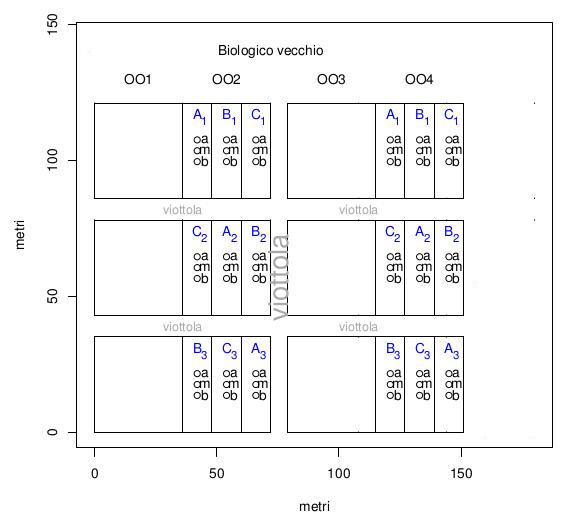
\includegraphics[width=0.75\textwidth]{../foto/OO_sito.jpeg}
  \caption{Appezzamenti biologico, i plot sono indicati con dei codici
    identificativi: \emph{OO} seguito da un numero che indica
    l'appezzamento; la lettera maiuscola indica la lavorazione
    \emph{A}(aratura), \emph{B}(rippatura), \emph{C}(frangizollatura);
    il numero (\emph{1, 2 , 3}) indica la riga; la lettera minuscola
    indica la replica all'interno del plot (\emph{a} alto, \emph{m}
    medio, \emph{b} basso) \label{fig:OO_sito}}
\end{figure}

\begin{figure}
  \centering
  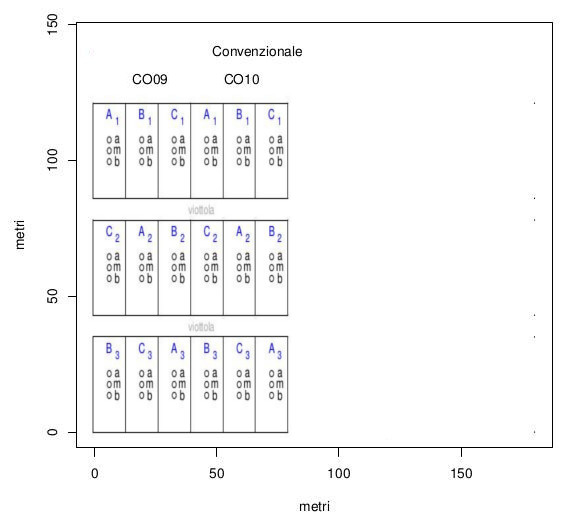
\includegraphics[width=0.75\textwidth]{../foto/CO_sito.jpeg}
  \caption{Appezzamenti convenzionale, la codifica segue quella
    descritta per l'appezzamento biologico \label{fig:CO_sito}}

\end{figure}


\section{Misura della densit\`a apparente}
L'ipotesi che ci ha portato ad effettuare questa misurazione \`e data
dal fatto che la conduzione biologica, non utilizzando concimi e
pesticidi di sintesi, avrebbe un minor impatto sulla microflora e
microfauna tellurica. Di conseguenza ci aspetteremmo una migliore
struttura con la conduzione biologica.  La densit\`a apparente
del suolo è stata misurata con il metodo \emph{Core} (utilizzando grandi
volumi) e con il metodo \emph{Clod} (utilizzando piccoli aggregati).

\subsection{Metodo \emph{Core}}%Densimetria per grandi volumi (cilindro)}
Per misurare la densit\`a apparente del suolo con il metodo della
pesata \citep{ugolini2010basi}, sono stati prelevati dei campioni di
terreno mediante l'utilizzo di un cilindro non deformabile di volume
noto (Fig. \ref{fig:cilindro}). \dubbio{verifica unit\`a di
  misura e metti una moneta accanto al cilindro per avere idea delle
  dimensioni}


\begin{figure}[ht]
  \centering
  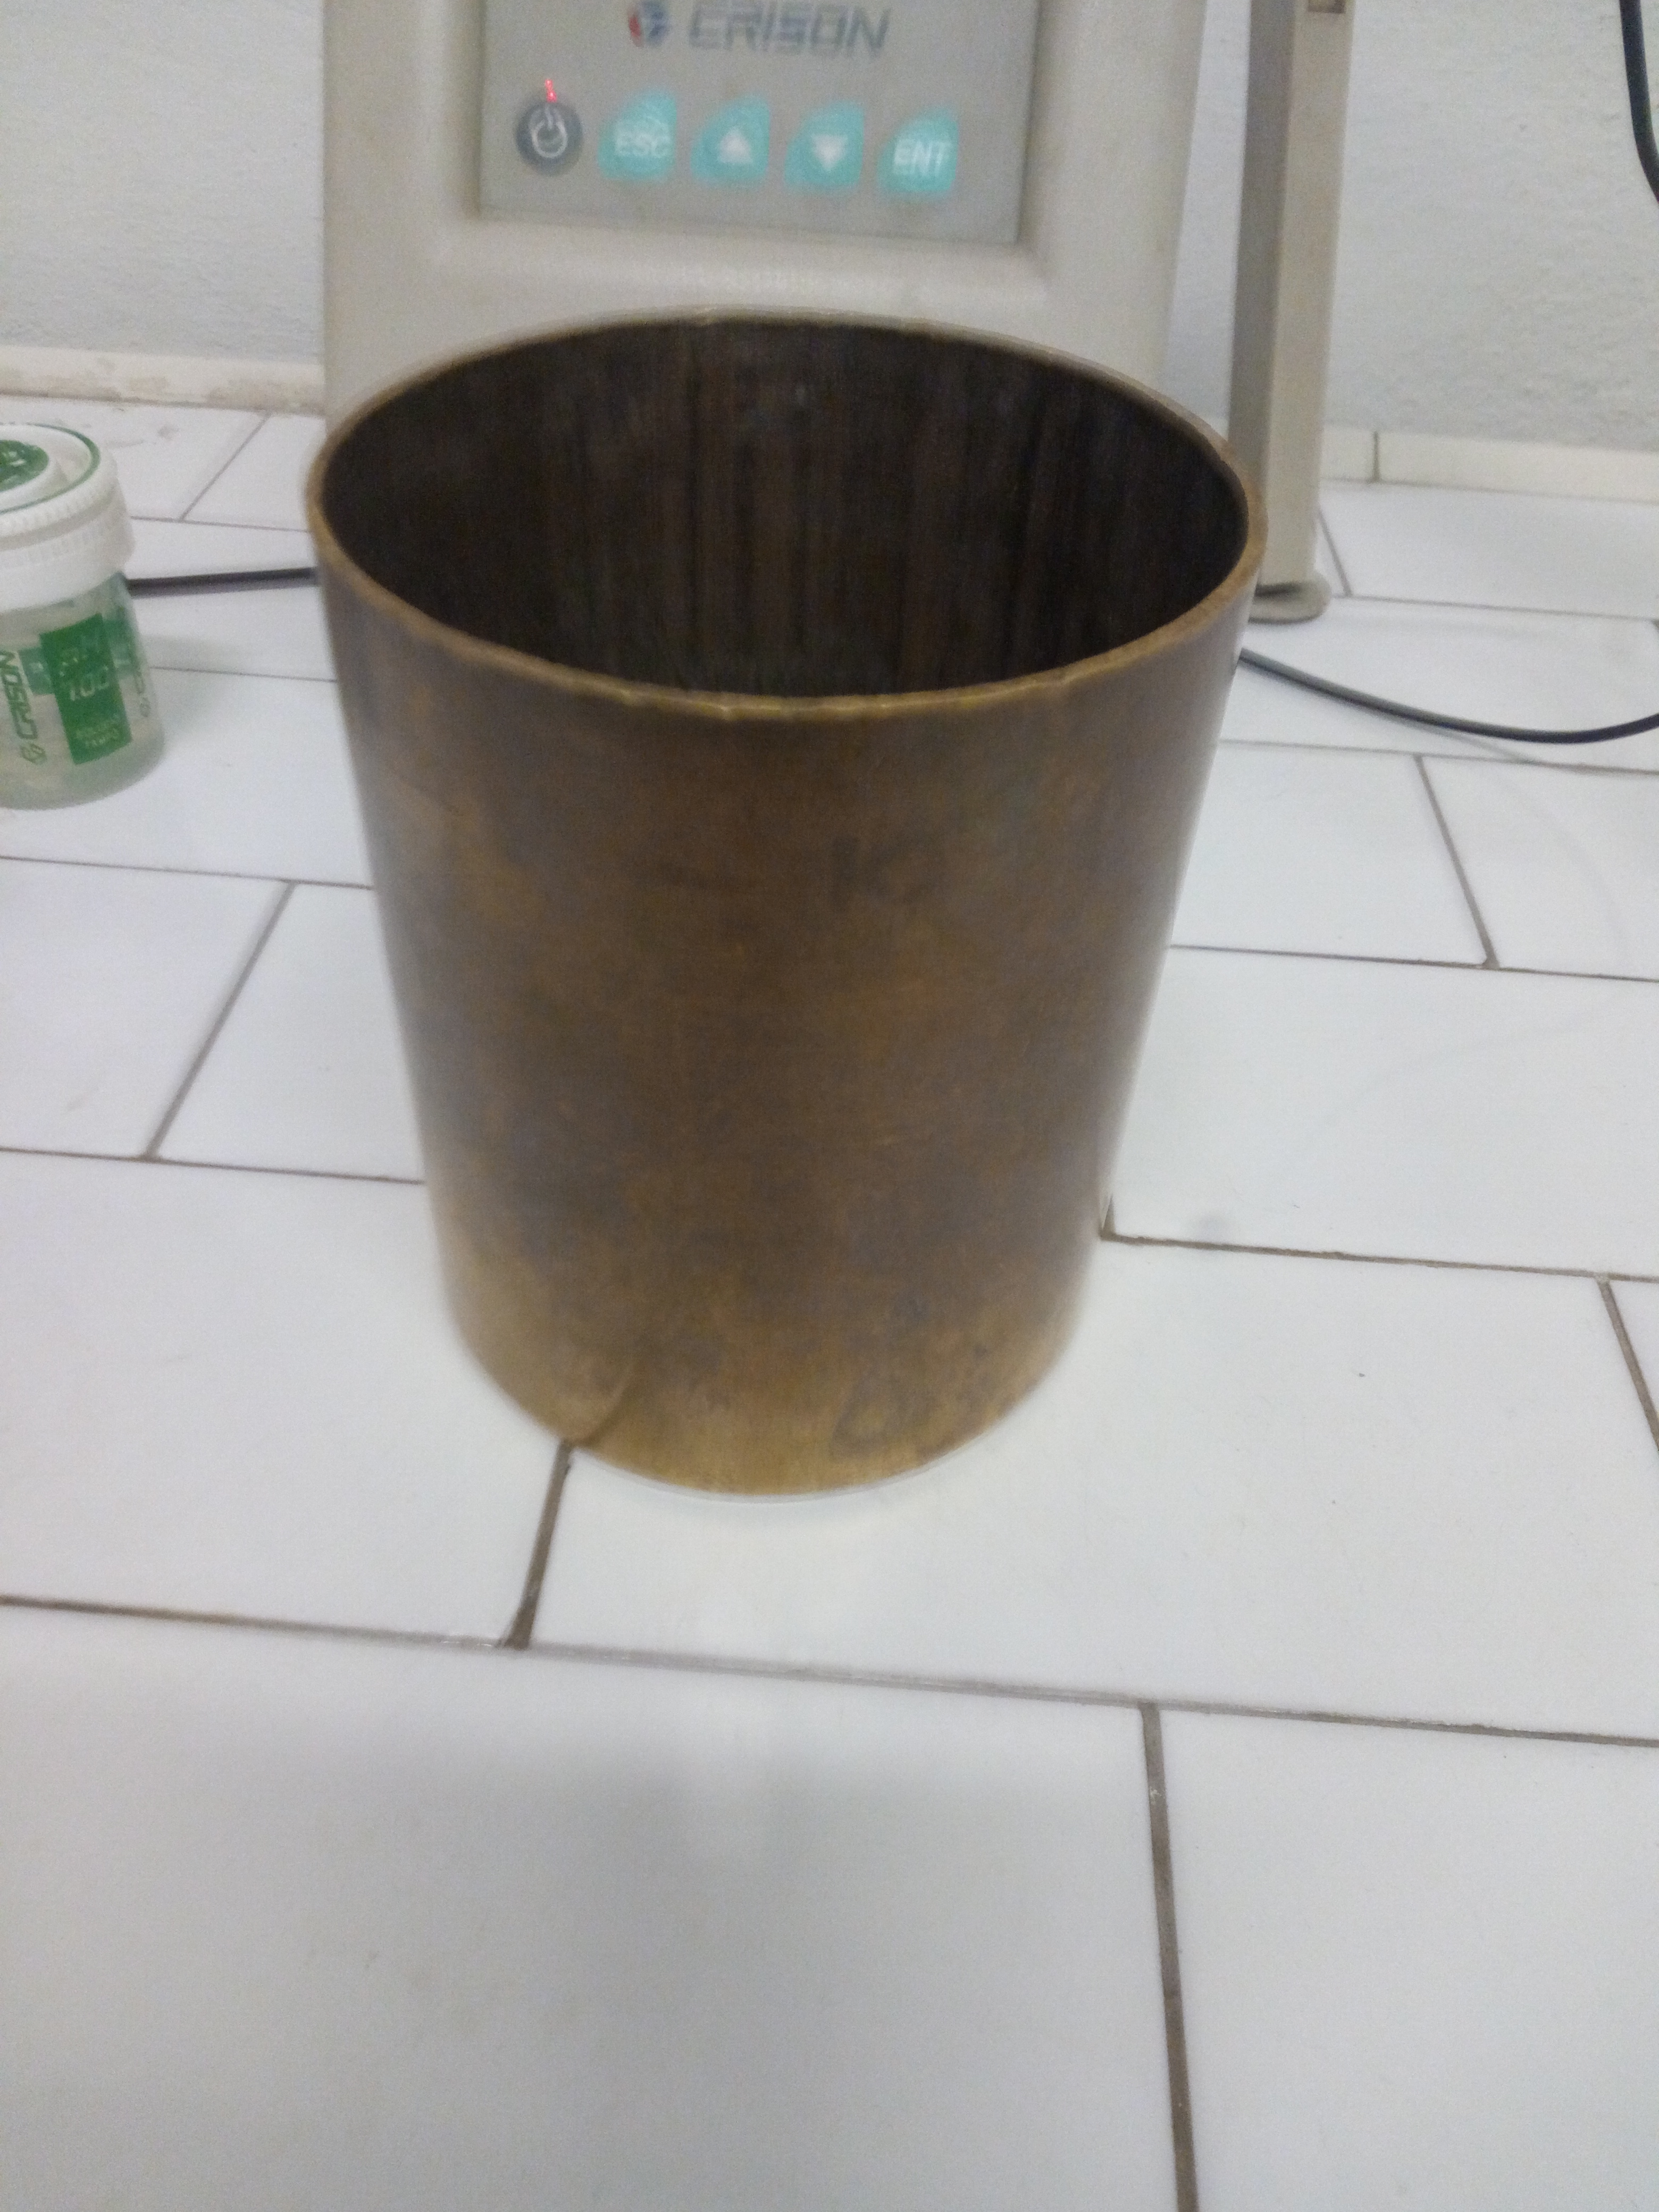
\includegraphics[width=0.5\textwidth]{../foto/cilindroOttone.jpeg}
  
  \caption{Cilindro in ottone utilizzato per prelevare i campioni da
    destinare all'analisi di densit\`a apparente col metodo
    \emph{Core}, altezza = \SI{12}{\centi\metre}
    diametro = \SI{9.5}{\centi\metre} }
  \label{fig:cilindro}
\end{figure}



Il cilindro \`e stato inserito nel suolo per tutta la sua lunghezza e
quindi estratto facendo attenzione che il materiale al suo interno non
esca in modo da formare due superfici piatte sulle basi del cilindro.
Il campione prelevato, portato in laboratorio, \`e stato passato a
umido attraverso un vaglio con fori circolari di \SI{2}{\milli\metre}
di diametro. Il volume dello scheletro rimasto nel vaglio \`e stato
misurato per spinta idrostatica.  Il suolo vagliato
\`e stato essiccato in stufa a \SI{105}{\celsius} fino a peso
costante, e successivamente pesato. 

\begin{figure}[ht]
  \centering
  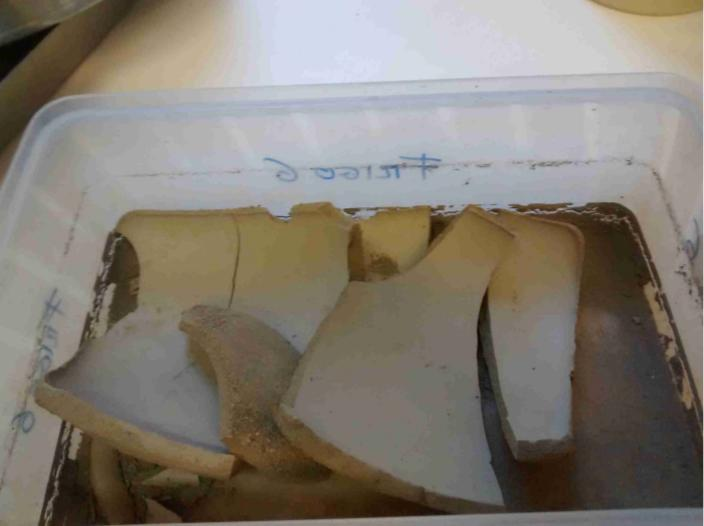
\includegraphics[width=0.8\textwidth]{../foto/secco.jpeg}
  \caption{\label{fig:secco}}
\end{figure}
Con i dati misurati, \`e stato ricavato il valore della densit\`a
apparente ($D_{App}$) tramite la seguente formula:
\begin{equation}
  \label{eq:DensitaApparente}
  D_{App}=\frac{P_{secco}}{V_{cil}-V_{scheletro}}
\end{equation}

Dove:\\
\begin{tabular}{rp{12cm}}
  $V_{cil}$=       & volume del cilindro di ottone (\SI{854.1}{\cubic\centi\metre}); \\
  $V_{scheletro}$=    & volume dello scheletro misurato per spinta
                        idrostatica espresso in \SI{}{\cubic\centi\metre}; \\
  $P_{secco}$=       & peso del terreno vagliato ed essiccato espresso
                       in \SI{}{\cubic\centi\metre}.
\end{tabular}
\vspace*{3em}




Questo lavoro di tesi \`e la prosecuzione di uno studio gi\`a
effettuato nell'anno 2015-2016 con le stesse modalit\`a. Per estendere
i risultati sono stati inclusi anche questi dati.



\subsection{Metodo \emph{Clod}}%Densimetria per piccoli aggregati (petrolio)

A differenza del metodo \emph{Core}, questa misura viene di solito
effettuata su aggregati di piccole dimensioni.  Il metodo \emph{Clod}
viene anche detto metodo per spinta idrostatica
\citep{Monnier_1973}. La procedura \`e consistita nel
mettere per una notte a bagno nel petrolio degli aggregati di
terreno (Fig. \ref{fig:petrolio}) cercando di ridurre al minimo le
manipolazioni per mantenere la struttura dell'aggregato stesso.

\begin{figure}[ht]
  \centering
  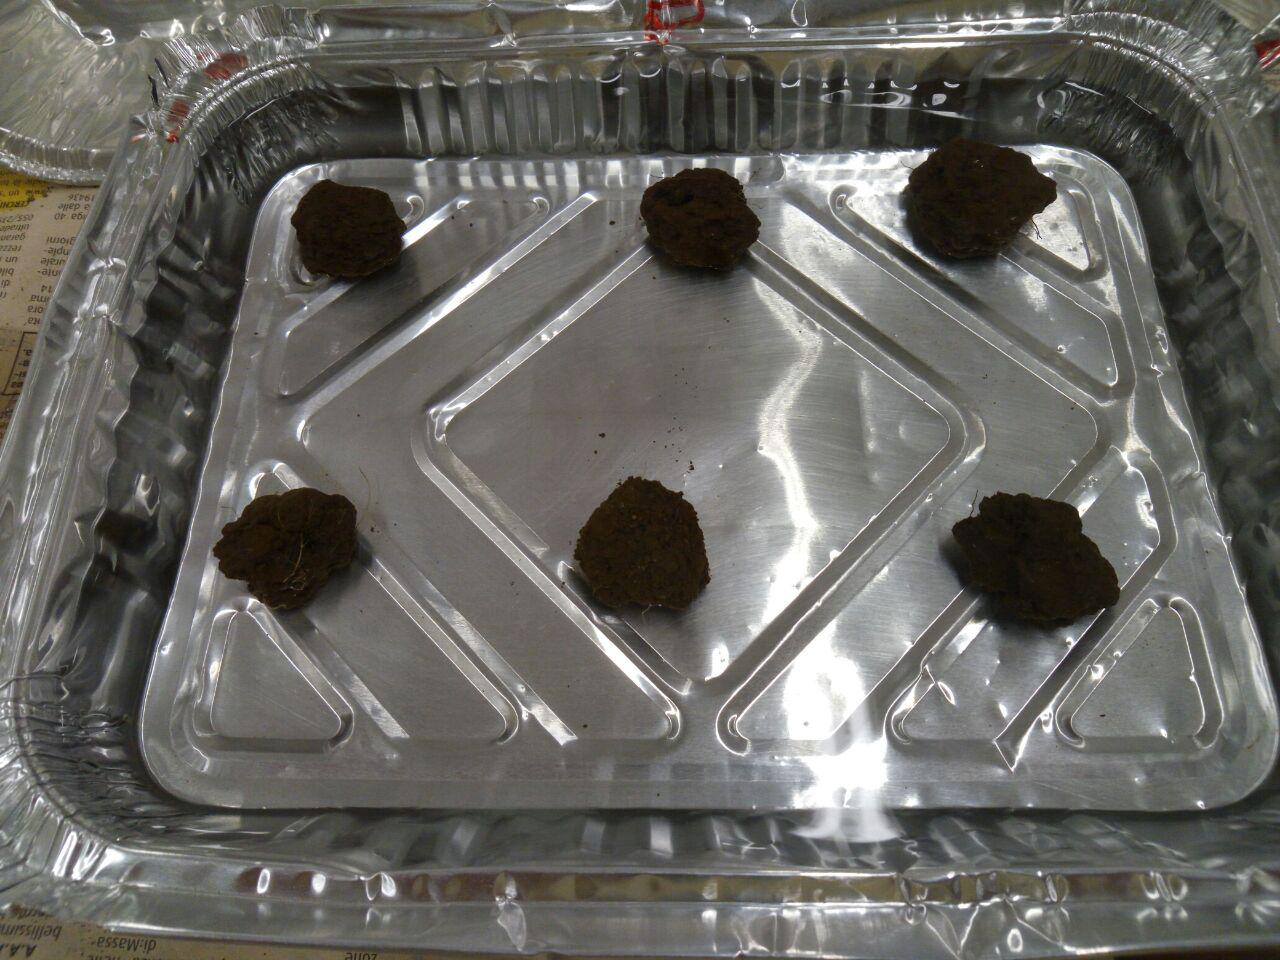
\includegraphics[width=0.8\textwidth]{../foto/petrolio.jpeg}
  \caption{\label{fig:petrolio}}
\end{figure}



Successivamente sono stati asciugati gli aggregati (completamente
imbevuti di petrolio) con carta, fino a "brillantezza", in modo che
solo una pellicola di liquido avvolgesse il campione. Per misurare la
spinta idrostatica \`e stato posto sul piatto di una bilancia precisa
al milligrammo, un contenitore riempito di petrolio nel quale era
immersa una navicella di rete forata, mantenuta da un supporto
metallico. Dopo aver misurato la tara, si \`e posto il campione entro
navicella (Fig. \ref{fig:bilancia}) e si \`e misurato il peso del
petrolio spostato.

\begin{figure}[ht]
  \centering
  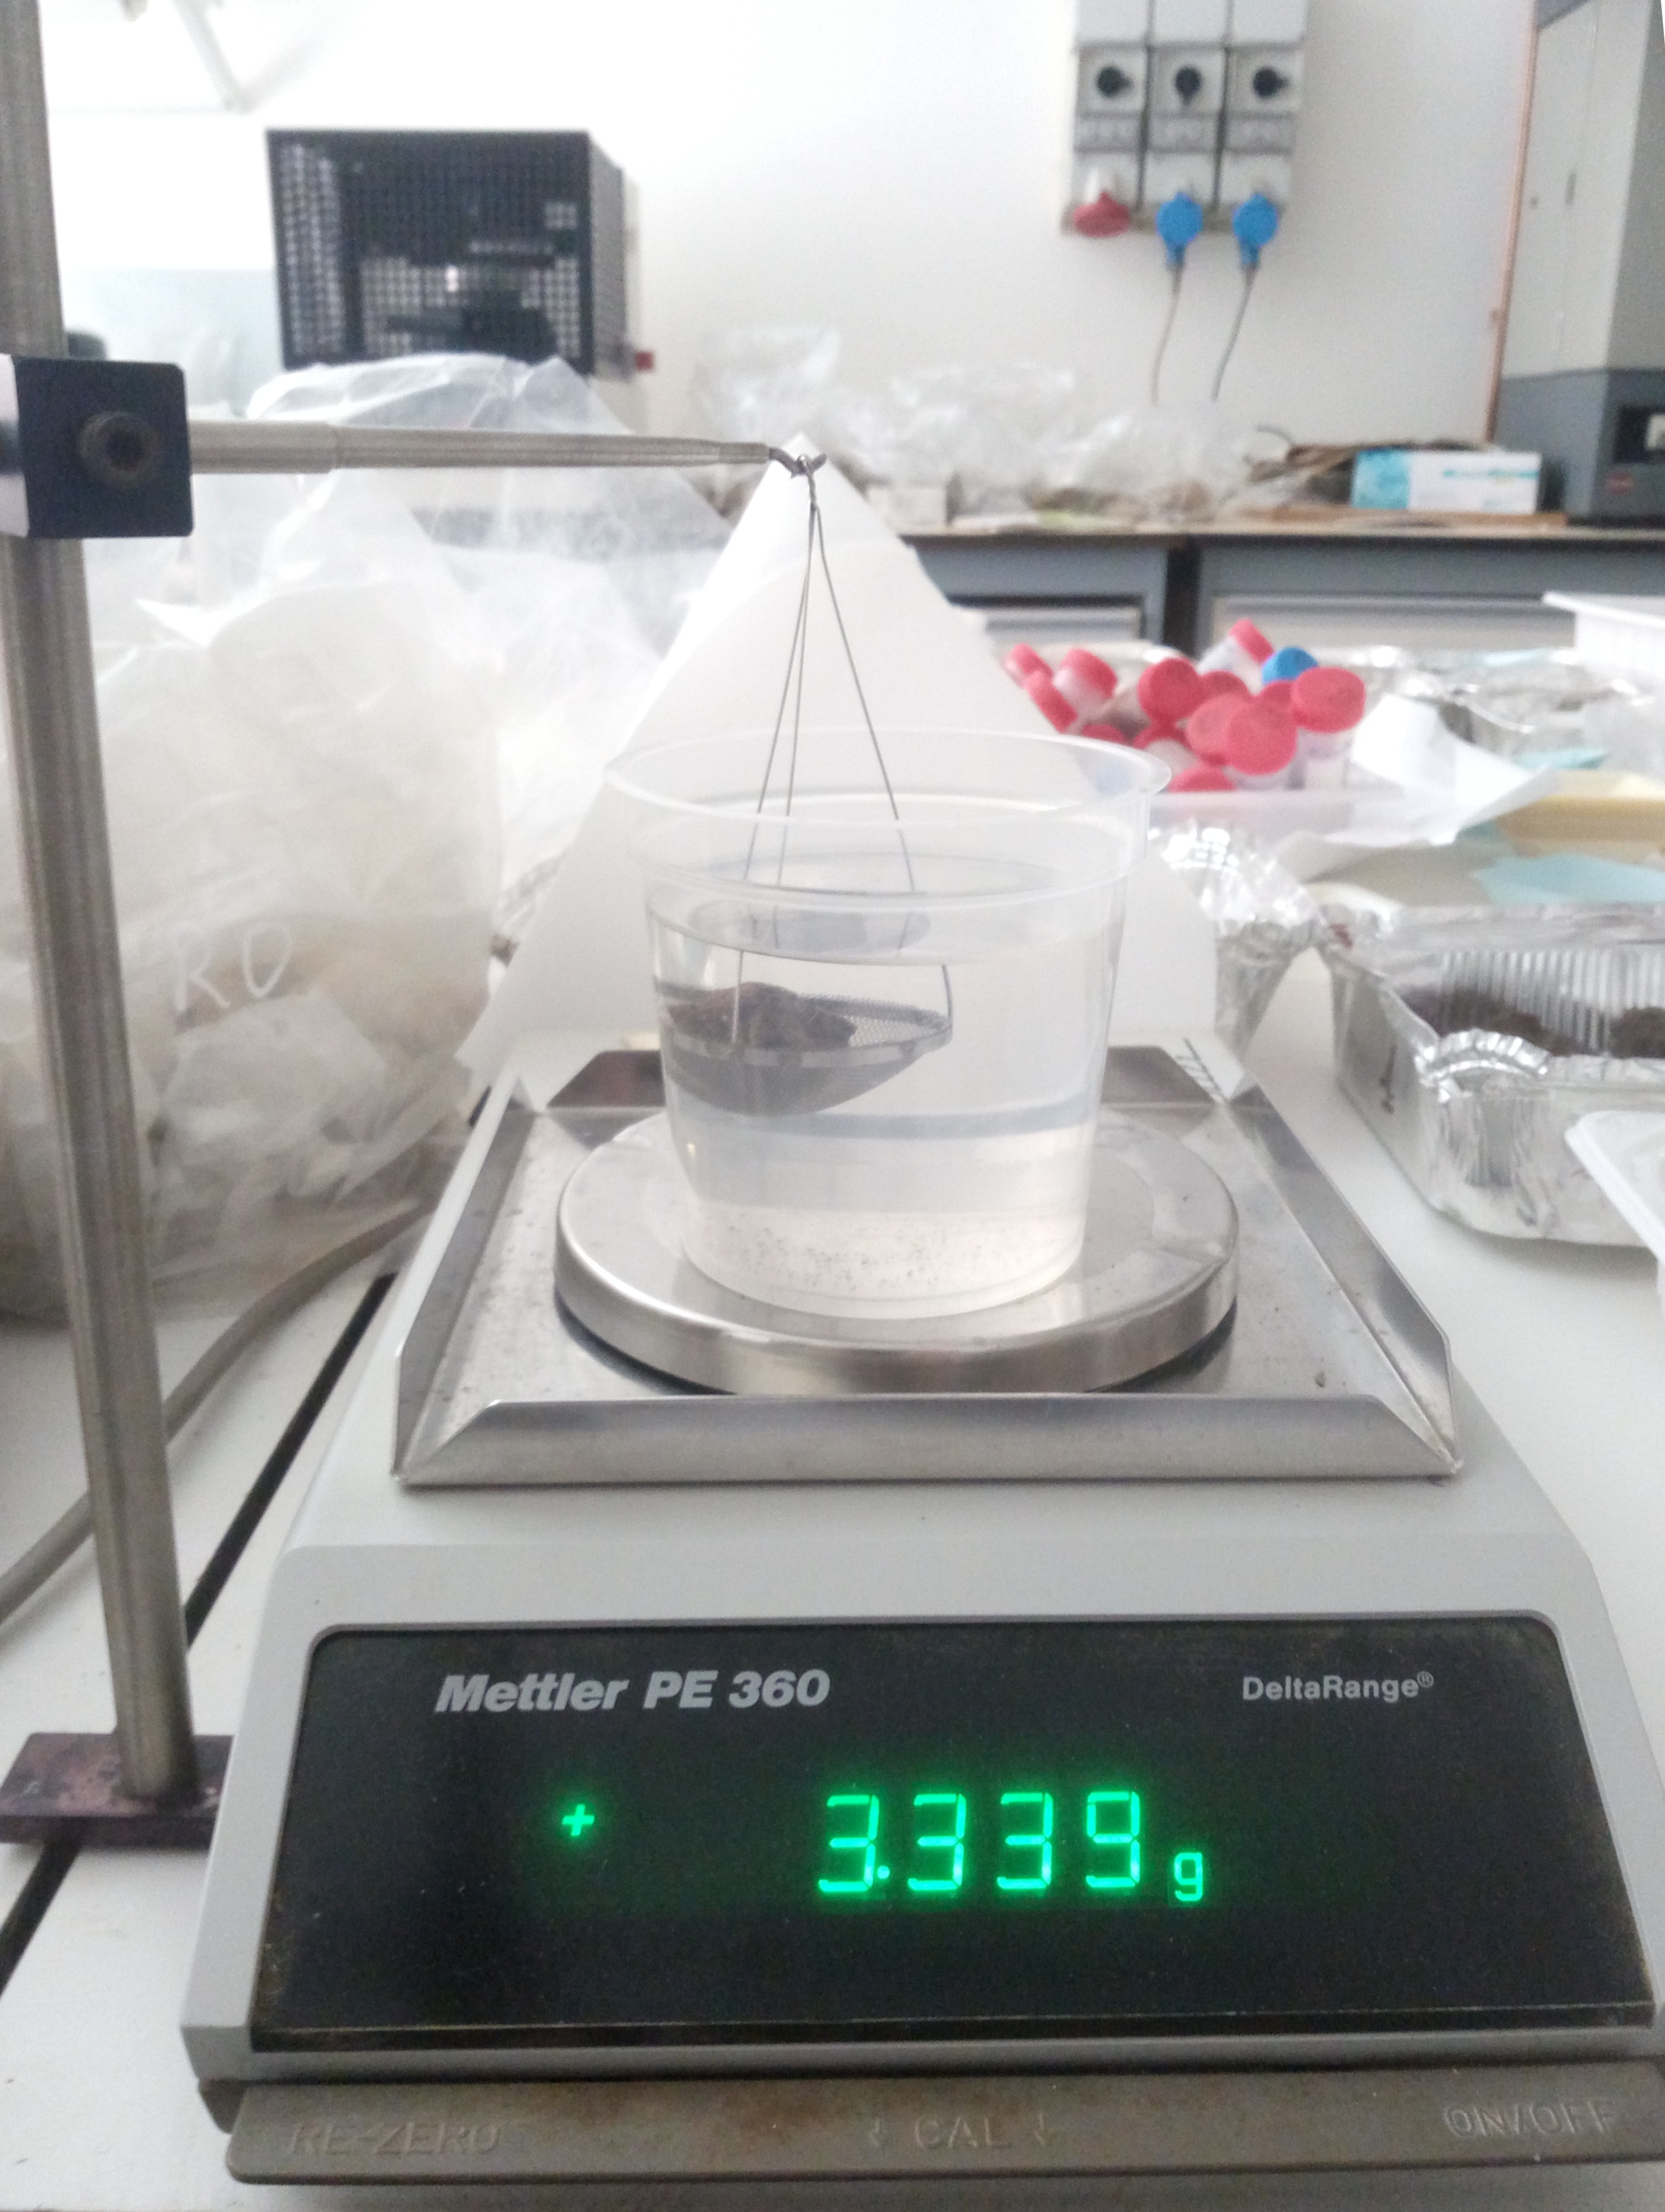
\includegraphics[width=0.8\textwidth]{../foto/navicella.jpeg}
  \caption{\label{fig:bilancia}}
\end{figure}

Per il principio di Archimede, il peso misurato \`e uguale al peso del
volume di petrolio spostato, da questa informazione \`e stato
possibile calcolare al volume del campione applicando la seguente
formula:

\begin{equation}
  \label{eq:VolumeAggr}
  V_{aggregato}=\frac{P_{petrolio}}{D_{petrolio}}
\end{equation} 

Dove:\\
\begin{tabular}{rp{12cm}}
  $V_{aggregato}$= & volume dell'aggregato comprendente anche il
                    volume dei pori in \SI{}{\cubic\cm};\\
  $P_{petrolio}$=  &  valore della spinta idrostatica
                   dell'aggregato imbevuto di petrolio in \SI{}{\gram};\\
  $D_{petrolio}$=  &  densit\`a del petrolio utilizzato per
                  l'analisi (\SI{0.761}{\gram\per\cubic\cm}).
\end{tabular}


Successivamente il campione \`e stato essiccato per una notte a
\SI{150}{\degreeCelsius} \footnote{Il raggiungimento di questa
  temperatura consente di allontanare l'acqua di idratazione dei
  cationi di scambio bivalenti (Ca, Mg) degli interstrati dei minerali
  a reticolo espandibile \citep{Monnier_1973}} quindi \`e stato
pesato. Il peso misurato \`e quello della fase solida.


Per calcolare la densit\`a reale \`e stato diviso il peso del campione
essiccato a \SI{150}{\celsius} con il volume del petrolio spostato dal
campione calcolato con il metodo precedentemente descritto:

\begin{equation}
  \label{eq:densitapetrolio}
  D_{App} = \frac{P_{150}}{V_{aggregato}}
\end{equation}

Dove:\\
\begin{tabular}{rp{12cm}}
  $D_{apparente}$=  & Valore della densit\`a apparente dell'aggregato
                       misurato in \SI{}{\gram\per\cubic\cm};\\
  $P_{150}$=       & peso dell'aggregato essiccato a
                     \SI{150}{\celsius} espresso in \SI{}{\gram};\\
  $V_{aggregato}$=  & volume calcolato con la formula
                      \ref{eq:VolumeAggr} espresso in \SI{}{\cubic\cm}.
\end{tabular}

Questo tipo di misura fornisce dei valori di densit\`a apparente pi\`u
elevati rispetto a quelli misurati utilizzando il cilindro, questo \`e
dovuto al fatto che nella misura non sono considerate le fratture
\citep{tisdall1951comparison}.

\subsection{Elaborazione dei dati \label{modello}}
I dati sono stati analizzati utilizzando il linguaggio di
programmazione ad oggetti R 3.4.0 \citep{r_programming}.

Per entrambi i metodi di analisi, \emph{Clod} e \emph{Core}, \`e stato
adattato un modello lineare additivo nella forma:
\info[inline]{Bugia. Nel Clod manca l'anno 2015 ! Non importa se lo dici dopo. I modelli son diversi}

\[
Y \sim \mu + \beta_1x_1 + \beta_2x_2 + \beta_3x_3 + \epsilon
\]

dove: \\ 

\begin{tabular}{rp{12cm}}
  $\beta_1 =$ & anno, due livelli: 2015, 2016;\\
  $\beta_2 =$  & conduzione, due livelli: convenzionale, biologico;\\
  $\beta_3 =$ & lavorazioni, tre livelli: arato, rippato, frangizollato;\\
  \info[inline]{$\epsilon =$ ??.}
               
\end{tabular}
\vspace*{3em}

La variabile categorica \emph{anno}, \`e stata utilizzata
solamente per l'analisi col metodo \emph{Core},
in quanto solo per questa sono disponibili dati dell'anno 2015.

\migliora[inline]{L'esplorazione dei modelli è stata fatta mediante
  confronto di modelli marginali, formalmente codificata con un test F: }


Entrambi i modelli sono stati validati attraverso l'analisi
esplorativa dei residui in modo da verificare le eventuali violazioni
delle assunzioni di normalit\`a \citep{stefanini2007introduzione}.

Successivamente per verificare la significativit\`a dei
trattamenti, \`e stata effettuata una analisi della varianza (ANOVA).
% di II tipo (package "car")<- in realt\`a no, però boh.
con valore prefissato $P < 0.05$.

Per una ulteriore verifica, ai gruppi oggetto dello studio \`e stato
applicato il test di Siegel-Tukey utilizzando i pacchetti 'agricolae'
\citep{agricolae} e 'multcomp' \citep{multcomp}.




\section{Distribuzione dinamica della dimensione degli aggregati}
La dinamica di disgregazione degli aggregati di suolo \`e stata
indagata per mezzo dello strumento Mastersizer 2000 \citep{Mas_2000}.
Il Mastersizer 2000 \`e mostrato in Fig. \ref{fig:Mastersize2000}
nella cui didascalia vengono descritti i dettagli.
\begin{figure}[ht]
  \centering
  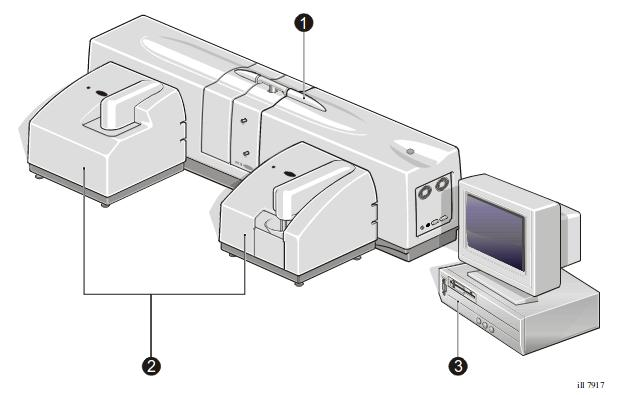
\includegraphics[width= \textwidth]{../foto/mastersizer.jpeg}
  \caption{Schema dello strumento Mastersizer 2000,
    immagine tratta dal manuale utente.  1) un tavolo ottico, che
    colleziona i dati i quali verranno usati per calcolare la
    dimensione delle particelle del campione; 2) una unit\`a di
    dispersione del campione, che ha lo scopo di disperdere il
    campione in acqua e mandarlo al tavolo ottico tramite una pompa;
    3) un elaboratore su cui è installato il software apposito che
    analizza i dati grezzi per determinare la dimensione delle
    particelle.\label{fig:Mastersize2000}}
\end{figure}

Il Mastersizer 2000 dispone di un emettitore di
ultrasuoni utile a rompere gli aggregati.

Nel nostro caso, la presenza di una pompa e di un agitatore che
applicano energia al campione (attraverso il ricircolo dell'acqua)
sono fondamentali per la determinazione della resistenza alla
disgregazione degli aggregati. Infatti effettuando una lettura a
intervalli regolari (quindi analizzando la variazione della
distribuzione nel tempo) \`e possibile determinare la capacit\`a degli
aggregati di resistere a sollecitazioni meccaniche.

\info{La parte che stava qui è stata spostata all'appendice}
\subsection{Protocollo di misura}
Da una aliquota dei campioni freschi \`e stata separata una
frazione di suolo compresa tra 1 e \SI{2}{\milli\meter} e,
successivamente, seccata a \SI{40}{\celsius}.  Prima della misurazione
effettiva del campione \`e necessario misurare il "bianco" per
acquisire $I_0$ (equazione \ref{eq:BeerLambert}). 

Da questa aliquota, \SI{300}{\mg} sono stati immessi
nell'unit\`a di dispersione del campione opportunamente riempita di
acqua.  Lo strumento effettua una misurazione della distribuzione
granulometrica ogni minuto, per 12 minuti. Al tempo stesso provvede al
ricircolo dell'acqua che disgrega le particelle.  Dal
\SI{13}{\degree} al \SI{24}{\degree} minuto, per completare la rottura
degli aggregati, viene attivata la sonicazione.

\subsection{Distribuzione granulometrica dinamica}
A conclusione della misura abbiamo ottenuto, per ogni campione, 48
distribuzioni granulometriche, in particolare:
\begin{itemize}
\item 12 distribuzioni dal minuto 1 al minuto 12 per il campione secco
  senza sonicatura;
\item 12 distribuzioni dal minuto 13 al minuto 24 per il campione
  secco con la sonicatura attiva;
\item 12 distribuzioni dal tempo 1 al tempo 12 per il campione umido
  senza sonicatura;
\item 12 distribuzioni dal minuto 13 al minuto 24 per il campione
  secco con la sonicatura attiva.
\end{itemize}

\begin{figure}[ht]
  \centering
  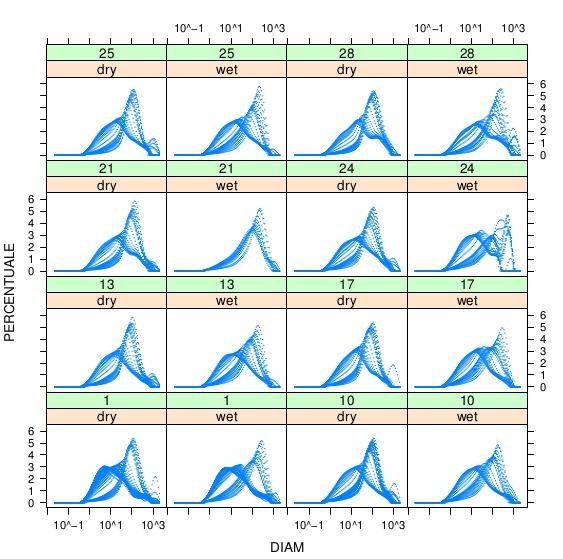
\includegraphics[width=0.8\textwidth]{../foto/distropisa.jpeg}
  \caption{In figura alcuni esempi di curve di distribuzione
    granulometrica dinamica: sull'asse delle ascisse sono presenti i valori dei
  diametri delle varie particelle misurate dallo strumento in
  \SI{}{\micro\metre}, scala logaritmica; sull'asse delle ordinate
  sono presenti i relativi valori di volume in percentuale sul totale.}
\end{figure}

\section{Porosimetria}

\section{Elaborazione dei dati}
I dati provenienti da queste analisi sono, per loro stessa natura,
composizionali e quindi sono stati analizzati con il package R
'Composition' \citep{compositional}.  I valori in output dagli
strumenti, infatti, sono espressi come valore percentuale sul totale.

Questi sono stati raggruppati in tre range dimensionali (macro
aggregati, meso aggregati, micro aggregati e macro pori, meso pori,
micro pori). Le dimensioni sono state definite in base alla
letteratura \citep{la letteratura}.

Da qui in poi, per la verifica di significativit\`a delle ipotesi, si
\`e proceduto come nel caso dell'analisi della densit\`a apparente,
ovvero con la costruzione del modello (opportunamente validato
mediante esplorazione visuale dei residui) e quindi con l'analisi
della varianza.


\chapter{Risultati}
\section{Densit\`a apparente}


\subsection{Metodo \emph{Core}}

La tabella \ref{tab:riassunto_1} riassume i dati ottenuti calcolando
la densit\`a apparente mediante la formula
\ref{eq:DensitaApparente}. La figura \ref{fig:boxplotCore} riporta gli
stessi dati in forma grafica. I valori, la cui media generale \`e pari a
\SI{1.38}{\gram\per\cubic\centi\metre}, 
non si allontanano
molto da quelli che pi\`u frequentemente si riscontrano nel suolo,
ovvero circa la met\`a della densit\`a reale che si aggira intorno a
\SI{2.65}{\gram\per\cubic\centi\metre}


% latex table generated in R 3.4.1 by xtable 1.8-2 package
% Tue Aug 22 10:59:37 2017
\begin{table}[hb]
\centering
\caption{Valori medi della densit\`a apparente (in \SI{}{\gram\per\cubic\centi\metre}), condizionati per anno, conduzione e lavorazione } 
\label{tab:riassunto_1}
\begin{tabular}{lllccc}
  \hline
Anno & Management & Tillage & Media & Dev. std & n \\ 
  \hline
2015 & Co & Ara & 1.35 & 0.14 &   5 \\ 
    &   & Fzo & 1.34 & 0.07 &   5 \\ 
    &   & Rip & 1.38 & 0.10 &   5 \\ 
    & Or & Ara & 1.37 & 0.10 &  15 \\ 
    &   & Fzo & 1.44 & 0.10 &  15 \\ 
    &   & Rip & 1.43 & 0.07 &  15 \\ 
  2016 & Co & Ara & 1.38 & 0.16 &   6 \\ 
    &   & Fzo & 1.35 & 0.15 &   6 \\ 
    &   & Rip & 1.26 & 0.09 &   5 \\ 
    & Or & Ara & 1.37 & 0.06 &   6 \\ 
    &   & Fzo & 1.35 & 0.07 &   6 \\ 
    &   & Rip & 1.40 & 0.15 &   6 \\ 
   \hline
\end{tabular}
\end{table} \FloatBarrier

 \info[inline]{Dobbiamo giustificare la differenza di numerosità del campione; 5, 6, 15,. Propongo di far sparire quei 15 e portarli a 5}
La figura \ref{fig:boxplotCore} mostra che l'anno 2015 \`e presenta
una densit\`a apparente mediamente pi\`u elevata dell'anno 2016. Non
sono visibili differenze tra le varie lavorazioni, ma si nota come i
valori di densit\`a apparente misurati sul campo convenzionale siano
pi\`u bassi rispetto a quelli del biologico.



\begin{figure}[hb]
  \centering
\includegraphics{Tesi_GIT-figboh2}

\caption{Boxplot della densit\`a apparente per i vari trattamenti: 
  a sinistra sono presenti le misurazioni dell'anno 2015, a destra quelle del 2016; 
  all'interno dei due anni sono suddivisi in Convenzionale e Organico; 
  per colore si possono distinguere le varie lavorazioni (arato, frangizollato e rippato);
  \info[inline]{La riga rossa ?}
  }
  
  \label{fig:boxplotCore}
\end{figure}
\FloatBarrier


Il modello utilizzato, \`e quello descritto alla sotto sezione
\ref{modello}. \`E stato costruito un modello additivo in quanto non
sono state trovate interazioni statisticamente significative tra
l'anno, la conduzione e la lavorazione.

La tabella \ref{tab:anova del modello} riporta l'Anova del
modello. L'anova mostra che il valore di p dell'effetto della lavorazione
sui dati \`e sopra a 0.05 (valore prefissato di significativit\`a), di
conseguenza si pu\`o eliminare dal modello. Mentre l'anno e la
conduzione sono statisticamente significative.


% latex table generated in R 3.4.1 by xtable 1.8-2 package
% Tue Aug 22 10:59:38 2017
\begin{table}[ht]
\centering
\caption{Tabella ANOVA per i valori di densità rilevati col metodo \emph{Core}} 
\label{tab:anova del modello}
\begin{tabular}{rrrrrr}
  \hline
 & Df & Sum Sq & Mean Sq & F value & Pr($>$F) \\ 
  \hline
Anno & 1 & 0.05 & 0.05 & 4.36 & 0.0395 \\ 
  Conduzione & 1 & 0.05 & 0.05 & 4.68 & 0.0332 \\ 
  Lavorazione & 2 & 0.01 & 0.00 & 0.26 & 0.7702 \\ 
  residui & 90 & 0.97 & 0.01 &  &  \\ 
   \hline
\end{tabular}
\end{table}
In tabella \ref{tab:t-table del modello2} \`e possibile vedere la
t-table del modello senza la variabile categorica lavorazione
\info[inline]{Mi pare si fosse detto che si chiamava tillage}.

Da questa \`e possibile confermare ci\`o che \`e stato mostrato
dall'analisi visuale, ovvero: il terreno degli appezzamenti condotti a
biologico \`e mediamente pi\`u denso di quello degli appezzamenti
condotti a convenzionale. Inoltre l'anno 2015 presenta delle densit\`a
apparenti pi\`u alte rispetto all'anno 2016.



% latex table generated in R 3.4.1 by xtable 1.8-2 package
% Tue Aug 22 10:59:38 2017
\begin{table}[ht]
\centering
\caption{} 
\label{tab:t-table del modello2}
\begin{tabular}{rrrrr}
  \hline
 & Estimate & Std. Error & t value & Pr($>$$|$t$|$) \\ 
  \hline
Co 2015 & 1.36 & 0.02 & 62.28 & 0.00 \\ 
  Scostamento 2016 & -0.03 & 0.02 & -1.52 & 0.13 \\ 
  Scostamento Or & 0.05 & 0.02 & 2.18 & 0.03 \\ 
   \hline
\end{tabular}
\end{table}


\begin{figure}[ht]
  \centering 
\includegraphics{Tesi_GIT-figboh}
\caption{Boxplot densit\`a apparente in cui \`e stato eliminato
  l'effetto della lavorazione dal modello, le lettere sopra ai boxplot
  sono il risultato del test di Tukey-Siegel \info[inline]{al livello
    di significatività ??}}
\end{figure}
\FloatBarrier

In conclusione di questa analisi, i dati non permettono di confermare
l'ipotesi di partenza.

Tuttavia la differenza tra la densit\`a apparente del terreno condotto
a biologico e quello condotto a convenzionale non \`e significativa a
livello tecnologico, infatti la differenza \`e al livello della
seconda cifra decimale. Questo per\`o ci permette di affermare che il
disegno sperimentale \`e ben costruito e che il numero di campioni \`e
sufficiente per gli obiettivi dello studio.
\info{forse questa roba va messa nel capitolo discussione}

\subsection{Metodo \emph{Clod}}
Con il metodo \emph{Clod}, grazie alla speditivit\`a del metodo sono
stati analizzati tutti i 108 campioni disponibili, ogni misura \`e
stata replicata tre volte.

In tabella \ref{tab:summary petrolio} sono riportati in sintesi
le informazioni presenti nel data frame. \`E possibile vedere come i
valori della densit\`a apparente calcolati (mediante l'equazione
\ref{eq:densitapetrolio}) siano mediamente pi\`u elevati rispetto a
quelli dell'analisi col metodo \emph{Core}.

% latex table generated in R 3.4.1 by xtable 1.8-2 package
% Tue Aug 22 10:59:39 2017
\begin{table}[ht]
\centering
\caption{Valori medi della densit\`a apparente (in 
                \SI{}{\gram\per\cubic\centi\metre}), 
                condizionati per conduzione e lavorazione } 
\label{tab:summary petrolio}
\begin{tabular}{llccc}
  \hline
Management & Tillage & Media & Dev. std & n \\ 
  \hline
Co & Ara & 1.93 & 0.06 &  18 \\ 
   & Fzo & 1.89 & 0.05 &  18 \\ 
   & Rip & 1.90 & 0.06 &  18 \\ 
  Or & Ara & 1.90 & 0.07 &  18 \\ 
   & Fzo & 1.84 & 0.06 &  18 \\ 
   & Rip & 1.87 & 0.07 &  18 \\ 
   \hline
\end{tabular}
\end{table}


Dai boxplot mostrati in Fig. \ref{fig:boxplotpetrolio} non sono visibili
differenze tra i trattamenti.


\begin{figure}[ht]
  \centering 
\includegraphics{Tesi_GIT-figmah}
\caption{Boxplot dei valori di densit\`a apparente ottenuti col metodo
  di analisi \emph{Clod}; gli appezzamenti condotti convenzionalmente
  (a sinistra) hanno valori leggermente più alti degli appezzamenti
  condotti a biologico (a destra) le lettere sopra ai boxplot sono il
  risultato del test di Tukey-Siegel \info[inline]{al livello di
    significatività ??}}
  \label{fig:boxplotpetrolio}

\end{figure}

Il modello \`e additivo; come nel caso del metodo \emph{Core} le
interazioni tra lavorazione e conduzione non sono statisticamente
significative.

I trattamenti sono statisticamente significativi come si pu\`o vedere
dalla tabella Anova del modello (tabella \ref{tab:anova piccoli aggregati}).


% latex table generated in R 3.4.1 by xtable 1.8-2 package
% Tue Aug 22 10:59:41 2017
\begin{table}[ht]
\centering
\caption{} 
\label{tab:anova piccoli aggregati}
\begin{tabular}{rrrrrr}
  \hline
 & Df & Sum Sq & Mean Sq & F value & Pr($>$F) \\ 
  \hline
Management & 1 & 0.03 & 0.03 & 6.31 & 0.0135 \\ 
  Tillage & 2 & 0.05 & 0.02 & 5.83 & 0.0040 \\ 
  Residui & 104 & 0.42 & 0.00 &  &  \\ 
   \hline
\end{tabular}
\end{table}
La t-table (tabella \ref{tab:sommario piccoli aggregati}) mostra come i
terreni a conduzione biologica abbiano una densit\`a apparente minore
rispetto a quelli convenzionali; il terreno in cui \`e stata
effettuata l'aratura, \`e indicato come pi\`u denso rispetto ai
terreni rippati e frangizollati.



% latex table generated in R 3.4.1 by xtable 1.8-2 package
% Tue Aug 22 10:59:41 2017
\begin{table}[ht]
\centering
\caption{} 
\label{tab:sommario piccoli aggregati}
\begin{tabular}{rrrrr}
  \hline
 & Estimate & Std. Error & t value & Pr($>$$|$t$|$) \\ 
  \hline
Co Arato & 1.93 & 0.01 & 157.38 & 0.00 \\ 
  Scostamento Or & -0.03 & 0.01 & -2.51 & 0.01 \\ 
  Scostamento Frangizollato & -0.05 & 0.02 & -3.39 & 0.00 \\ 
  Scostamento Rippato & -0.03 & 0.02 & -2.04 & 0.04 \\ 
   \hline
\end{tabular}
\end{table}
Come nel metodo \emph{Core}, anche in questo caso il numero di campioni
\`e stato sufficiente a determinare la differenza significativa di due
trattamenti nonostante si differenzino per la seconda cifra decimale.




\section{Distribuzione dinamica della dimensione degli aggregati}






%% \migliora{ref aitchinson, analisi of compositional data, buccianti e
   
%%    egozcue mettere nella discussione come mai si usano i composizionali
 
%%    mettere nei matmet il modello usato mettere 10 alla meno 3 nella tabella 3.7

%%    didascalia estesa in figura 3.4}


Per la costruzione dei modelli sono stati esclusi i trattamenti
lavorazione, che non sono significativi, Nel modello \`e presente
l'elemento tempo al quadrato il quale, come \`e possibile vedere dalla
tabella anova \ref{tab:anova_compWET}, \`e significativo.

La misura \`e stata effettuata sia sull'aggregato secco che
sull'aggregato inumidito per studiare il fenomeno dello
\emph{slaking} \footnote{Rottura di
aggregati di suolo (>2-\SI{5}{\mm}) secchi in aggregati pi\`u piccoli
(<\SI{0.25}{\mm}) quando sono improvvisamente immersi in acqua. Lo
slaking avviene quando gli aggregati non sono forti abbastanza da
resistere agli stress interni causati dal rapido ingresso dell'acqua
\citep{Slaking}}.  \dubbio{E invece il suolo wet si distrugge prima
  ahah. Non torna niente.}  Quindi sono stati creati due modelli: uno
per i campioni inumiditi (\emph{WET}) e uno per i camioni secchi
(\emph{DRY}). I modelli mostrano che pendenza e curvatura sono comuni
per entrambi i trattamenti.

Alla fine del trattamento, \`e possibile vedere come tutti gli
aggregati in fondo al trattamento disgregativo (acqua + ultrasuoni)
mostrino distribuzioni granulometriche uguali.

I paletti macro meso micro sono a 150, rispettivamente
\info{mettere i valori sulle figure}. Giustificare anche come mai si
sono scelti questi valori invece che sab lim arg (io 8rino non me lo
ricordo)

La curvatura non ci interessa se non come un modo per estrarre
informazione dai dati.

I secchi generano, come atteso, particelle più grandi in seguito allo
slacking \info{E invece dovrebbe essere esattamente il contrario,
  visto che lo slaking distrugge gli aggregati grandi e li riduce in
  briciole.}
  
Risulta che gli aggregati provenienti da appezzamenti condotti
convenzionalmente, non appena vengono lasciati cadere in acqua, si
disgregano generando particelle più grosse di quanto non facciano gli
aggregati "biologici". E questo avviene sia con aggregati umidi che
secchi.

Siccome le particelle inizialmente liberate sono anch'esse mantenute
insieme da cementi che vengono distrutti in seguito, possiamo
concludere che i cementi presenti nella conduzione biologica sono
leggermente, ancorch\`e significativamente, meno efficaci nel
mantenere la struttura del suolo.




% latex table generated in R 3.4.1 by xtable 1.8-2 package
% Tue Aug 22 10:59:42 2017
\begin{table}[ht]
\centering
\begin{tabular}{lllll}
  \hline
Conduzione & Fase & Macro (\%) & Meso (\%) & Micro (\%) \\ 
  \hline
Convenzionale & inizio misura & 43.8 & 41.9 & 14.3 \\ 
    & inizio sonicatura & 17.9 & 32.9 & 49.2 \\ 
    & fine misura & 8.4 & 10.6 & 81 \\ 
   &  &  &  &  \\ 
  Biologico  & inizio misura & 39 & 44.7 & 16.4 \\ 
    & inizio sonicatura & 14.9 & 32.7 & 52.5 \\ 
    & fine misura & 6.7 & 10.2 & 83.1 \\ 
   \hline
\end{tabular}
\caption{Progressione della distribuzione delle particelle 
                  liberatisi dagli aggregati precedentemente inumiditi in seguito a: 
                  i) immersione:
                  ii) inizio sonicazione 
                  iii) fine  } 
\label{tab:iufw}
\end{table}

% latex table generated in R 3.4.1 by xtable 1.8-2 package
% Tue Aug 22 10:59:42 2017
\begin{table}[ht]
\centering
\caption{Progressione della distribuzione delle particelle 
                  liberatisi dagli aggregati secchi in seguito a: 
                  i) immersione:
                  ii) inizio sonicazione 
                  iii) fine  } 
\label{tab:iufd}
\begin{tabular}{lllll}
  \hline
Conduzione & Fase & Macro (\%) & Meso (\%) & Micro (\%) \\ 
  \hline
Convenzionale & inizio misura & 61.8 & 22.8 & 15.3 \\ 
    & inizio sonicatura & 19.1 & 25.9 & 55 \\ 
    & fine misura & 8.5 & 11.8 & 79.7 \\ 
   &  &  &  &  \\ 
  Biologico  & inizio misura & 57.3 & 24.8 & 17.9 \\ 
    & inizio sonicatura & 16.1 & 25.5 & 58.4 \\ 
    & fine misura & 6.9 & 11.2 & 81.8 \\ 
   \hline
\end{tabular}
\end{table}
% latex table generated in R 3.4.1 by xtable 1.8-2 package
% Tue Aug 22 10:59:42 2017
\begin{table}[ht]
\centering
\caption{anova stabilit\`a aggregati per i dati WET } 
\label{tab:anova_compWET}
\begin{tabular}{rrrrrrr}
  \hline
 & Df & Pillai & approx F & num Df & den Df & Pr($>$F) \\ 
  \hline
Intercetta & 1 & 0.92 & 4955.26 & 2 & 835 & 0.0000 \\ 
  Management & 1 & 0.09 & 41.72 & 2 & 835 & 0.0000 \\ 
  Tempo & 1 & 0.92 & 4504.77 & 2 & 835 & 0.0000 \\ 
  Tempo\verb|^|2 & 1 & 0.35 & 227.06 & 2 & 835 & 0.0000 \\ 
  Residui & 836 &  &  &  &  &  \\ 
   \hline
\end{tabular}
\end{table}


% latex table generated in R 3.4.1 by xtable 1.8-2 package
% Tue Aug 22 10:59:42 2017
\begin{table}[ht]
\centering
\caption{Aggregati per i dati WET } 
\label{tab:anova_compWET}
\begin{tabular}{rrrrrrr}
  \hline
 & Df & Pillai & approx F & num Df & den Df & Pr($>$F) \\ 
  \hline
Intercetta & 1 & 0.88 & 3047.17 & 2 & 857 & 0.0000 \\ 
  Management & 1 & 0.12 & 59.60 & 2 & 857 & 0.0000 \\ 
  Tempo & 1 & 0.92 & 5153.70 & 2 & 857 & 0.0000 \\ 
  Tempo\verb|^|2 & 1 & 0.30 & 183.27 & 2 & 857 & 0.0000 \\ 
  Residui & 858 &  &  &  &  &  \\ 
   \hline
\end{tabular}
\end{table}



\begin{figure}[ht]
  \centering 
\includegraphics{Tesi_GIT-figboh3}
  \caption{Plot del modello composizionale}
\end{figure}


\begin{figure}[ht]
  \centering 
\includegraphics{Tesi_GIT-figboh4}
  \caption{qqplot del modello composizionale \info[inline]{quale ???}}
  \label{fig:qqplot_dinamica_aggregati}
\end{figure}

\section{Porosimetria}

\info{Ho messo intanto tutto l'import, poi per i grafici aspetto il prof}

\chapter{Discussione}

Dall'analisi statistica \`e emerso che  
\section{Dati composizionali: cosa sono e come vengono analizzati
  \citep{van2013analyzing}}

\info{Mi faccio un riassuntino dell'introduzione del libro intanto}
Tradizionalmente un dataset pu\`o essere definito composizionale se
contiene porzioni di totale: percentuale di lavoratori in differenti
settori, porzioni di elementi chimici in un minerale, tessitura di un
suolo ecc.

Le parti individuali delle composizioni sono chiamate
\emph{componenti}. Ogni \emph{componente} ha una quota (in valori
  assoluti o relativi), rappresentata dalla sua importanza sul totale.

I metodi classici di analisi multivariata sono inapplicabili per i dati
composizionali che richiedono, quindi, il loro set di metodi
statistici e non dovrebbero essere trattati con metodi fatti per dati
scalari \citep{aitchison1986statistical}.

La caratteristica fondamentale dei dati composizionali \`e che non
siamo interessati alla somma totale delle composizioni, questo accade
per diverse ragioni:
\begin{itemize}
  \item quando i dati composizionali sono misurati, possiamo
    influenzare il totale;
   \item spesso il totale delle composizioni non \`e completo e non dà
     la somma del totale "reale";
   \item tipicamente, il totale non \`e comparabile tra le diverse
     unit\`a statistiche.
\end{itemize}

Una composizione \`e sempre formata da pi\`u subcomposizioni. E la
stessa composizione di partenza \`e a sua volta una subcomposizione:
infatti i dati composizionali non possono contenere ogni singola parte
dell'unit\`a statistica analizzata.

Nonostante ci\`o, l'analisi dei dati composizionali \`e eseguibile
anche su dataset a cui mancano delle componenti irrilevanti, questa
\`e chiamata 'coerenza subcomposizionale'
\citep{aitchison1986statistical}.

I dati composizionali vengono sempre trattati in una
\emph{log-ratio-transformed scale}. Questo operazione porta a definire
uno spazio vettoriale ristretto, contenuto nello spazio reale,
denominato \emph{simplesso}.

In questo spazio vettoriale possono essere applicate tutte le tecniche
di statistica multivariata ai dati composizionali trasformati; i
risultati verranno anti-trasformati in composizioni per poter essere
interpretabili.

\chapter{Conclusioni}

\chapter{Prospettive}

\begin{appendices}
\chapter{Calcolo della concentrazione delle componenti granulometriche con Mastersizer 2000}
Il Mastersizer 2000 si basa sul fenomeno della diffusione ottica (scattering), ovvero
\textit{un'ampia classe di fenomeni di interazione radiazione-materia
  in cui onde o particelle vengono deflesse ovvero cambiano
  traiettoria) a seconda della collisione con altre particelle o onde
  (dal punto di vista quantistico) in maniera disordinata e in buona
  maniera casuale} \citep{scattering}.  

Le equazioni che descrivono lo scattering sono molto complesse; nel
caso in cui le particelle abbiano dimensione maggiore della lunghezza
d'onda della radiazione luminosa incidente, esiste (assumendo la
perfetta sfericit\`a delle particelle) una soluzione matematicamente
rigorosa, detta \textit{Soluzione di Mie}.

\begin{figure}[ht]
  
\includegraphics[width=\textwidth]{../foto/Mie_scattering.jpeg}
  \caption{In figura \`e rappresentato il fenomeno dello scattering di Mie, presa da
    \href{http://www.smart-piv.com/en/techniques/mie-rayleigh-raman/index.php}{questo
      sito}
    \label{fig:Mie}}
\end{figure}

Se la dimensione delle particelle e dettagli riguardanti la loro
struttura sono noti, il modo in cui diffondono la luce pu\`o essere
previsto accuratamente. Ogni dimensione della particella avr\`a il suo
caratteristico pattern di diffusione che sar\`a diverso da quello di
qualsiasi altra particella a diversa dimensione.

Facendo il ragionamento inverso \`e quindi possibile calcolare la
dimensione delle particelle in base al pattern di diffusione.

\begin{figure}[ht]
  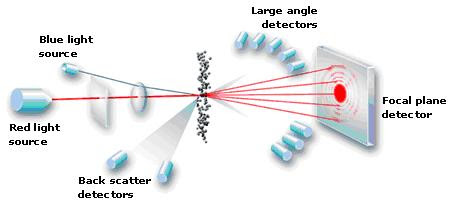
\includegraphics[width=\textwidth]{../foto/laser_diffraction.jpeg}
  \caption{Rappresentazione del funzionamento del Mastersizer 2000 presa da:
    \href{https://plus.google.com/communities/110676150876604729660/stream/ffa7f40a-1c65-4268-9121-bb88d63f0c41}{questo sito}
    \label{fig:MastersizerInt}}
\end{figure}
Per calcolare la concentrazione del campione, il software utilizza la
legge di \textit{Lambert-Beer}: 

\begin{equation}
  \label{eq:BeerLambert}
  \frac{I}{I_0}=e^{-\alpha b}
\end{equation}

Dove:\\
\begin{tabular}{rp{12cm}}
  $I$            & è l'intensit\`a della luce a una distanza $b$ dal campo
                   delle particelle di assorbanza $\alpha$\\
  $I_0$          & è l'intensit\`a della radiazione luminosa all'ingresso
                   del campo delle particelle \\
  $\frac{I}{I_0}$ & è la trasmittanza T del raggio (misurata direttamente dallo strumento), ovvero, $I_0$ \`e
                    l'intensit\`a del laser quando
                    nessun campione \`e presente e $I$ \`e l'intensit\`a con il
                    campione presente.
\end{tabular}

Esprimendo la legge in termini di trasmittanza e ri-arrangiando:

\begin{equation}
  \alpha=\frac{-1}{b}Ln \langle T \rangle
\end{equation}

Il termine $\alpha$ contiene informazioni riguardo la concentrazione e
la dimensione delle particelle. 

Dalla teoria dello scattering, la luce attenuata da una particella
$i$ pu\`o essere descritta da:

\begin{equation}
  a_i=Q_i\pi r_i^2n_i
  \label{eq:boh}
\end{equation}

Dove:\\
\begin{tabular}{rp{12cm}}
  $Q_i$& è l'efficienza dell'estinzione luminosa calcolata dalla
         teoria Mie per una particella di raggio $r_i$\\
       &Il secondo termine \`e l'area della sezione della particella
         e il termine finale $n_i$ \`e il numero di particelle di raggio $r_i$
\end{tabular}

In termini di volume delle particelle $V_i=\frac{4}{3}\pi r_i^3n_i$,
l'equazione \ref{eq:boh} diventa, per un insieme di particelle:

\begin{equation}
  \alpha_i=\frac{3}{4} \sum \frac{Q_iV_i}{r_i}
\end{equation}

La dimensione delle particelle \`e espressa in base al diametro $d$ e
il volume pu\`o essere separato in una distribuzione relativa dei
volumi $v$ e in una concentrazione totale $C_v$ (volume totale delle
particelle in una unit\`a di volume del disperdente). L'equazione
quindi diventa:

\begin{equation}
  \alpha_i=\frac{3}{2} \sum \frac{Q_iV_i}{d_i}
\end{equation}

Sostituendo con $\alpha$

\begin{equation}
  C_v=\frac{-2 Ln \langle T \rangle}{3b \sum \frac{Q_iv_i}{d_i}}
\end{equation}

Se $d$ \`e espressa in $\mu$m e b in mm, allora $v$ \`e la
concentrazione relativa della distribuzione del volume (in cui $\sum
v_i=1$) allora:

\begin{equation}
  \label{eq:boh2}
  C_v(ppm)=\frac{-2000 Ln \langle T \rangle}{3b \sum \frac{Q_iv_i}{d_i}}
\end{equation}

Questa equazione ci fornisce la concentrazione delle particelle di
dimensione $x_i$ in parti per milione
(ppm). Per calcolare il valore della percentuale di concentrazione del
volume, il valore finale deve essere diviso per 10000. 

Nell'equazione \ref{eq:boh2}:

\begin{tabular}{rp{12cm}}
  $\langle T \rangle$ &  Trasmittanza, \`e un valore compreso tra 0 e 1 ed \`e
          misurato direttamente dallo strumento\\
  $v_i$ & \`e la distribuzione di particelle, ovvero il volume relativo
          nella classe dimensionale $i$ con diametro medio $d_i$\\
  $Q_i$, & il coefficiente di estinzione medio per la classe
           dimensionale $i$, \`e calcolato dalla teoria dello scattering, ed
           \`e una funzione delle propriet\`a ottiche delle particelle e del
           mezzo disperdente.
\end{tabular}

\end{appendices}



\printbibliography
\listoftodos
\end{document}
